%%%%%%%%%%%%%%%%%%%%%%%%%%%%%%%%%%%%%%%%%%%%%%%%%%%%%%%%%%%%%%%%%%%%%%%%%%%%%%%%
%%%%%%%%%%%%%%%%%%%%%%%%%%%%%%%%%%%%%%%%%%%%%%%%%%%%%%%%%%%%%%%%%%%%%%%%%%%%%%%%
%                                                                              %
%       This is the beginning of a uothesisapa Dissertation                    %
%                                                                              %
%%%%%%%%%%%%%%%%%%%%%%%%%%%%%%%%%%%%%%%%%%%%%%%%%%%%%%%%%%%%%%%%%%%%%%%%%%%%%%%%
%%%%%%%%%%%%%%%%%%%%%%%%%%%%%%%%%%%%%%%%%%%%%%%%%%%%%%%%%%%%%%%%%%%%%%%%%%%%%%%%

\errorcontextlines 10000 % Get more logging information on errors. Following http://tex.stackexchange.com/a/83485/56363, if after setting this you see an error, "Note that the order is 'from inner to outer', that is, the first (non-indented) line is the point where the error actually occurred. The line after that (indented) is the part of that line which isn't yet processed, so the point of error is exactly at the line break."

%==============================================================================%
% Preamble
%==============================================================================%
% Options:
%     Pass a list of these separated by commas into the documentclass brackets
% Critical Options:
%     dissertation   - PhD Theses.
%     msthesis       - Master's Thesis
%     lackscommittee - no committee; often goes with Master's Thesis
%     copyright      - include copyright page. NOTE: You must customize this
%                      yourself under makecopyrightpage in uothesis.cls
%     final          - increases font size to 12pt, makes it twosided
%     approved       - Add the approval prefatory page (when you're done!)
% Extra Formatting Options:
%     sc             - use smallcaps instead of uppercase for chapter
%                      titles and stuff.
%     justified      - If you want to justify the text
%     bound          - Change for binding and printing. Does not comply with UO
%     amstex         - use amsmath, amssymb, amsthm Since it's in the .cls,
%                      they're bound early with RequirePackage. See also
%                      MATH EQUATIONS AND THEOREMS
%     chemistry      - use mhchem with ACS-style citations: superscript numbers
%                      for in-text citations with a numbered references cited
%                      section. Also loads mhchem.
%     apacite        - use APA style citations. If this is not included, you
%                      need to change this file a little; see the BIBLIOGRAPHY
%                      section.  You may also need to edit the makefile.
%     notables       - Do not include a "List of Tables" page
%     nofigures      - Do not include a "List of Figures" page
%     listings       - Include a "List of Source Code Listings" page. This
%                      requires you to add the following into this file:
%                    \usepackage{listings}
%                    \renewcommand{\lstlistoflistings}{\begingroup
%                    \tocfile{\lstlistingname}{lol}
%                    \endgroup}
% Notes:
%     - `draftcopy` is incompatible with `final`
%     - `msthesis` is incompatible with `dissertation`
%     - pick exactly one of `apacite`, `chemistry`, or nothing, if using a
%       custom citation style.
%     - ...and probably more.

% Examples:
\documentclass[dissertation, final, copyright]{uothesis} % For final copies

%\documentclass[dissertation, draftcopy]{uothesis} % For draft copies (enables line numbering, and puts black bars where there is text that overflows a line where latex can't figure out how to break it onto another line (in non-draft modes, this will result in an "overfull hbox" error, so draft mode is a good way of spotting these, following http://tex.stackexchange.com/a/39/56363)

%\documentclass[msthesis, lackscommittee, approved, final]{uothesis} % Example for Masters thesis that does not include a committee.

%------------------------------------------------------------------------------%
% PACKAGES
%------------------------------------------------------------------------------%
\usepackage[USenglish,UKenglish]{babel}
\usepackage{mathtools,amsmath,amsfonts,amsthm,amssymb,bm, bbm}
\usepackage{dcolumn,booktabs,longtable}
\usepackage[figurewithin=chapter,tablewithin=chapter]{caption}
%\usepackage[singlelinecheck=false]{caption}
%  \captionsetup[subfigure]{singlelinecheck=on, labelfont=normalfont}
%  \captionsetup[figure]{labelfont=it}
\usepackage{placeins}
\usepackage{graphicx}
\usepackage[space]{grffile} % allow spaces in graphics filenames.
\usepackage{rotating}
\usepackage{enumitem}
\usepackage{epstopdf}
\usepackage{ctable}
\usepackage{appendix}
\usepackage{setspace}
\usepackage[normalem]{ulem}
\usepackage{tabularx,xspace,multirow}
\usepackage{array}
\usepackage{caption}
\usepackage{subcaption}
\usepackage{listings}

% Added by Jacob L. following https://tex.stackexchange.com/questions/148314/undefined-control-sequence-in-printbibliography-biblatex to allow UTF-8 (non-ASCII) characters in the bibliography .bib file.
\usepackage[utf8]{inputenc}

%------------------------------------------------------------------------------%
% BIBLIOGRAPHY
%------------------------------------------------------------------------------%
%--- You need to specify these if your dissertation is something other than
%--- apacite+bibtex, but these may be helpful for anything nonstandard.
%
%--- For example: If using biblatex, you need to manually fix spacing and ensure
%--- bibitems do not straddle page breaks and show up in TOC
% \usepackage{bibspacing}
% \setcounter{secnumberdepth}{4}
% \patchcmd{\bibsetup}{\interlinepenalty=5000}{\interlinepenalty=10000}{}{}
% \setlength\bibitemsep{0.5\baselineskip}
% \usepackage{tocloft}
% \renewcommand{\cftchapfont}{\normalsize}
% \renewcommand{\cftchapleader}{\cftdotfill{\cftdotsep}} % for chapters
% \renewcommand*{\numberline}[1]{\hb{#1  \hfil}}
%
%--- Or, if you want to change the citation style to e.g. acm
% \bibliographystyle{acm}
% Use biblatex for references - change style= as appropriate
\usepackage[natbib=true,backend=biber,sorting=nyt,style=apa,sortcites=true]{biblatex}
\addbibresource{dissertation.bib}

%------------------------------------------------------------------------------%
% MATH EQUATIONS AND THEOREMS (.cls also restructures theorem layout)
%------------------------------------------------------------------------------%
%--- Change \align{} and \equation{} spacing
\usepackage{etoolbox}
\newcommand{\zerodisplayskips}{%
  \setlength{\abovedisplayskip}{3pt}
  \setlength{\belowdisplayskip}{3pt}
  \setlength{\abovedisplayshortskip}{3pt}
  \setlength{\belowdisplayshortskip}{3pt}}
\appto{\normalsize}{\zerodisplayskips}
\appto{\small}{\zerodisplayskips}
\appto{\footnotesize}{\zerodisplayskips}

\usepackage{lineno}
%\usepackage{authblk}
\usepackage{xparse}
\usepackage{xpunctuate}
\usepackage{wrapfig}

\usepackage[hidelinks]{hyperref}
\usepackage[all]{hypcap}
\usepackage{amsmath}
\usepackage{cleveref}
\usepackage{flafter}
\usepackage{floatrow}
\usepackage{cancel}
\usepackage{pdfpages}
\usepackage{lscape}
\usepackage{fancyhdr}% http://ctan.org/pkg/fancyhdr
\usepackage{bookmark}
\fancypagestyle{pdflandscape}{%
\fancyhf{}% Clear header/footer
  \fancyfoot{% Footer
    \makebox[\textwidth][r]{% Right
      \rlap{\hspace{\footskip}% Push out of margin by \footskip
        \smash{% Remove vertical height
          \raisebox{\dimexpr.5\baselineskip+\footskip+.5\textheight}{% Raise vertically
            \rotatebox{90}{\thepage}}}}}}% Rotate counter-clockwise
  \renewcommand{\headrulewidth}{0pt}% No header rule
  \renewcommand{\footrulewidth}{0pt}% No footer rule
}
%\usepackage[position=top, label font=bf,labelformat=simple]{subfig}
%%%
%\graphicspath{ {./figures/} }
%\floatsetup[figure]{style=plain, subcapbesideposition=top}
%\floatsetup[table]{style=Plaintop}
% local definitions
\newcommand{\msprime}[0]{\texttt{msprime}\xspace}
\newcommand{\tskit}[0]{\texttt{tskit}\xspace}
\newcommand{\slim}[0]{\texttt{SLiM}\xspace}
\newcommand{\pyslim}[0]{\texttt{pyslim}\xspace}
\newcommand{\stdpopsim}[0]{\texttt{stdpopsim}\xspace}
\newcommand{\allel}[0]{\texttt{scikit-allel}\xspace}
\newcommand*{\eg}{e.g.\xcomma}
\newcommand*{\ie}{i.e.\xcomma}
\NewDocumentCommand{\plcref}{m O{\empty}}{(\Cref{#1}{#2})}
\NewDocumentCommand{\lcref}{m O{\empty}}{\Cref{#1}{#2}}
\newcommand{\comment}[1]{}
\newcommand{\beginsupplement}{%
    \setcounter{table}{0}
    \renewcommand{\thetable}{S\arabic{table}}%
    \setcounter{figure}{0}
    \renewcommand{\thefigure}{S\arabic{figure}}%
}

\newcommand{\E}{\operatorname{E}}

\newcommand{\Var}{\operatorname{Var}}

\newcommand{\Cov}{\operatorname{Cov}}
\newcommand{\Cor}{\operatorname{Cor}}

\newcommand{\SD}{\operatorname{SD}}

\newcommand{\expnumber}[2]{{#1}\times10^{#2}}

\newcommand{\pianc}{\pi^{\mathrm{anc}}}

\def\fillandplacepagenumber{%
 \par\pagestyle{empty}%
 \vbox to 0pt{\vss}\vfill
 \vbox to 0pt{\baselineskip0pt
   \hbox to\linewidth{\hss}%
   \baselineskip\footskip
   \hbox to\linewidth{%
     \hfil\thepage\hfil}\vss}}


% from http://tex.stackexchange.com/questions/43648/why-doesnt-lineno-number-a-paragraph-when-it-is-followed-by-an-align-equation/55297#55297
\ifcsname{patchAmsMathEnvironmentForLineno}\endcsname
    \newcommand*\patchAmsMathEnvironmentForLineno[1]{%
      \expandafter\let\csname old#1\expandafter\endcsname\csname #1\endcsname
      \expandafter\let\csname oldend#1\expandafter\endcsname\csname end#1\endcsname
      \renewenvironment{#1}%
         {\linenomath\csname old#1\endcsname}%
         {\csname oldend#1\endcsname\endlinenomath}}%
    \newcommand*\patchBothAmsMathEnvironmentsForLineno[1]{%
      \patchAmsMathEnvironmentForLineno{#1}%
      \patchAmsMathEnvironmentForLineno{#1*}}%
    \AtBeginDocument{%
    \patchBothAmsMathEnvironmentsForLineno{equation}%
    \patchBothAmsMathEnvironmentsForLineno{align}%
    \patchBothAmsMathEnvironmentsForLineno{flalign}%
    \patchBothAmsMathEnvironmentsForLineno{alignat}%
    \patchBothAmsMathEnvironmentsForLineno{gather}%
    \patchBothAmsMathEnvironmentsForLineno{multline}%
\fi

\newcommand{\savenumberline}{}% reserve global name


%==============================================================================%
% PREFATORY PAGES
%==============================================================================%
% NOTE: When submitting the title to gradweb, it should end in a period. I know, it's weird.
\covertitle{The Main Title of the Dissertation: The Subtitle of the Dissertation}
\abstracttitle{The Main Title of the Dissertation: The Subtitle of the Dissertation}
\author{Hermione Granger}
\department{Department of Psychology}
\narrowdepartment{Department of Psychology}
\degreetype{Master of Philosophy}
\degreemonth{December}
\degreeyear{2021}
\chair{Albus Dumbledore}
\committee{Minerva McGonagall    & Core Member \\
           Severus Snape    & Core Member \\
           Sirius Black & Institutional Representative \\}
\graddean{Andy Karduna & Interim Vice Provost for Graduate Studies}

\abstract{
Evolutionary processes impact patterns of genetic variation,
so there is an opportunity to reverse this relationship and use genetic data to learn about past evolutionary events.
Traditional evolutionary inference from genetic data is plagued by a few issues:
(i) different processes can impact a particular feature in similar ways, 
making it difficult to disentangle them;
(ii) there is a growing need for modeling interactions between processes; and
(iii) many models do not make full use of genomic data and instead assume that loci are unlinked.

Simulation-based evolutionary inference can help alleviate many of these issues.
It is now possible to simulate complex evolutionary scenarios, 
and these can be used to approximate analytically intractable likelihoods,
for example by using supervised machine learning.
The major downsides to using simulations is the computational cost,
but recent advancements both in hardware and software have lessened this cost.
In this dissertation,
I pushed the boundaries on how simulation-based inference can be applied in evolutionary genetics.

To mitigate the costs associated with simulations,
I made a few contributions to the \tskit ecosystem of evolutionary simulation tools.
First, I developed a way to partially parallelize the simulation of multiple populations to make inference using multi-population genomic datasets more feasible.
Second, I helped create standards for reproducible simulations with natural selection within the \stdpopsim consortium.
I implemented the ability to simulate using previously published distribution of fitness effects (DFEs) and to simulate selective sweeps.
I demonstrate the utility of this tool by tackling the long-standing question of whether the power to detect sweeps varies along realistic chromosomes.

Next, I used simulations to better understand the behavior of a complex multi-population model.
Species can be thought as semi-independent realizations of the same (or very similar) evolutionary process.
Thus, by looking at multiple species at once it may be possible to better disentangle the processes that shape variation along genomes.
Using simulations, I show that positive selection is necessary to explain the genetic data obtained from multiple great ape species.
Further, I lay down a framework for leveraging multi-species information to better undestand the effects of different processes on a group's evolutionary history.

Lastly, I present a new method that uses whole-genome genealogies for evolutionary inference.
This data structure efficiently and sufficiently encodes evolutionary processes.
I develop a machine-learning framework, tsNN, that takes whole-genome genealogies as inputs
and is flexible enough to perform tasks at different scales (\eg inferring mutation times, demographic parameters, etc.).
I demonstrate that tsNN can learn to predict mutation times accurately, outperforming current likelihood-based methods.
tsNN, represents an important step in genealogy-based evolutionary inference, 
but there still much work to be done in applying deep learning to gain new insights into past evolutionary events.

}

\school{University of Oregon, Eugene, OR, USA}
\school{Universidade de São Paulo, São Paulo, SP, Brasil}

\degree{Doctor of Philosophy, Biology, 2024, University of Oregon}
\degree{Master of Science, Genetics and Evolutionary Biology, 2018, Universidade de São Paulo}
\degree{Bachelor of Science, Psychology, 2015, Universidade de São Paulo}

\interests{Evolutionary Biology}
\interests{Population Genetics}
\interests{Computational Biology}

\position{Graduate Employee, Data Carpentry, 2016}
\position{Graduate Affiliate, Digital Scholarship Center, University of Oregon, 2014-2016}
\position{Workshop Instructor (Archival Book Digitization, Scientific Programming in R, Scientific Programming with Version Control), Digital Scholarship Center and Department of Psychology, University of Oregon, 2015-2016}
\position{Instructor, Software Carpentry, 2014-2016}
\position{} % extra empty position is unnecessary

\award{Gregores Graduate Research Award, University of Oregon, 2013}
\award{Graduate School Research Award, University of Oregon, 2012}
\award{Marthe E. Smith Memorial Science Fellowship, University of Oregon, 2012}
\award{} % extra empty award is necessary

% Example publications:
\publication{Thomas, D. R. K., \& Smith, A. B. (2009). System models for the
             study of procrastination in high school students.
             \emph{American Journal of Everything}, 100, 7–20.}%
%\publication{Smith, A. B., Thomas, D. R. K., \& Kemper, S. (2008). Models and
%             instruments for analysis. E. Ramping \& J. R. Douglas (Eds.),
%             \emph{Behavior analysis: The areas of research} (pp. 67-69).
%             Englewood Cliffs, NJ: Prentice-Hall.}
\publication{} % extra empty publication is necessary

% The acknowledgements section is optional. It can cover at most two pages.
\acknowledge{
	% If don't have an acknowledgment, comment out or delete this whole file
	Here is an acknowledgment
}

  % acknowledgments page optional
% The dedication section is optional. It can cover at most one page.
\dedication{
	% If you don't have a dedication, comment out or delete this whole file
	To so-and-so\dots
}

        % dedication page optional



%==============================================================================%
% BEGIN DOCUMENT
%==============================================================================%
\begin{document}

% Following https://tex.stackexchange.com/a/313605, these two options will allow a rendered PDF to have the same checksum every time, because they suppress creation date and modification date info. from being written to the document.
\pdfinfoomitdate=1
\pdftrailerid{}

\maketitle



\chapter{Introduction}

\section{Decoding evolution: a lay-friendly prelude}
Evolution can occur over incredibly large spatial scales over the course of thousands to millions of years.
This makes Evolutionary biology unlike other fields within Biology in that hypotheses can not always be subject to experimentation.
Thus, we are left with the task of putting together what happened in the past based on information we have today.
To do so we need a sizable amount of data, models and statistical and computational tools.

One way to make inference about past evolutionary processes is by studying genetic variation within and between species.
Evolutionary processes, such as demographic processes, natural selection and mutation, impact the genetic variation in many ways.
For example, we expect the amount of variation within a species to be proportional to the mutation rate (\ie the higher the mutation rate, the more variation a population will harbor).
On the other hand, finite populations lose variation every generation due to genetic drift (\ie sampling error), 
and the magnitude of this loss is proportional to the population size.

We can write models in form of math equations that describe how some of these evolutionary processes impact genetic variation.
For example, $\pi$ (a metric of genetic variation) depends on the size of the population ($N$) and the mutation rate ($\mu$), such that $\pi \sim 4N\mu$.
If we knew the mutation rate, we could rearrange the equation to estimate the size of a population $N = \frac{\pi}{4\mu}$ from genetic data!
To arrive at this simple equation, we make the assumption that an individual is equally likely to mate with any other individual in the population (\ie panmixia).
It is easy to see how this may not always hold:
for example, a tree is much more likely to mate with another that lives close to it (because pollen cannot travel too far).

Adding biological realism to our math equation would prove to be complicated.
Alternatively, we can more easily simulate this process with a computer:
we can create virtual individuals and tell a computer how they choose their mates, pass on genetic material to their offspring, and change over time.
If we were to run virtual experiments like this many times,
it would be possible to map the relationship between genetic variation ($\pi$) and our parameters of interest (population size $N$ and mutation rate $\mu$).
This new map would be closer to the reality than our simplified mathematical model above,
but this approach is not a panacea, as simulations have a high computational cost (\ie they can take a long time to run).

For my dissertation, I have explored how we can incorporate computer simulations to help us understand evolution.
To this end, we need computational tools that are fast and reproducible (so that other researchers can use them).
So, in my second chapter, I discuss my contributions to tools that make these simulations run faster and to make them more reproducible.
Next, I gave my best to answer a long standing biological question: to what extent have humans and other apes been shaped by natural selection?
In my third chapter, I use simulations to tackle this question and show that both positive and negative selection are necessary to explain the genetic data obtained from multiple individuals for all great ape species.
Lastly, I wanted to build a proper statistical method that uses simulations to infer evolutionary processes from genetic data.
In my fourth chapter, I present a new method for evolutionary inference that uses genealogical trees along chromosomes (instead of tables with samples and mutations).
These trees capture the genetic data perfectly,
but they are much more scalable (use less space) and
they organize the data in a way that could be more conducive to extracting relevant evolutionary information.

\section{The current landscape in evolutionary inference}

% What are the major questions in evolutionary genetics?
Many questions in evolutionary biology are of a historical nature,
because evolution is restrict in space and time and it cannot be replicated.
An avenue for investigating past evolutionary events and processes lies in genetic data.
As evolutionary processes leave footprints on the genetic composition of populations,
the possibility arises to invert this relationship,
that is to use genetic data for the inference of past events.
Indeed, much of the field of evolutionary genetics is tasked with trying to infer past evolutionary events and processes from genetic data.
Some of the major questions the field has been interested in are:
Is it possible to find regions of the genome that were affected by natural selection?
Can we infer the movement of individuals and changes in population sizes over time?
What are the relative contributions of different evolutionary processes, such as demography and selection, in shaping patterns of genetic variation? 


% What challenges are in the way of answering these questions?
It has become clear that these questions cannot be investigated independently.
That is, to find regions of the genome under selection you need to understand the demographic history of populations,
and to infer demography from genetic data it is necessary to understand the effects of selections on genomes.
It is not possible to investigate each process in isolation because
(i) different processes can impact genetic variation in similar ways,
and (ii) modelling interactions between processes is not trivial.

% What kinds of signatures do evol processes leave on genetic data?
Inferring demographic processes from genetic data usually entail figuring out how these processes impact the underlying genealogies.
For example, if a population suddenly goes through a major bottleneck, we expect to see most of the coalescences concentrated during the bottleneck period.
On the other hand, population expansions can lead to trees that have coalescences concentrated in the period before the population expansion.
The underlying genealogies yield different patterns of genetic variation in the extant population.
One summary of genetic data that can be used to distinguish between these tree shapes and, in turn, between possible demographies is the site frequency spectrum (SFS).
The SFS is the distribution of allele frequencies across sites in some sampled genomes.
(For the sake of simplicity, I will focus on the unfolded SFS, where the frequency of the derived alleles have been measured; derived allele refers to the allele that is new to a population, which can be established by finding the ancestral allele with outgroups).
A genealogy that has coalescences concetrated at the tips (due to a recent bottleneck) will yield a SFS that is skewed towards the high frequency of derived alleles.
Conversely, a genealogy with coalescences happening earlier on will yield a SFS in which derived alleles are rare.

% Natural selection and the ways it impacts genetic variation
Natural selection also affect coalescence rates and shapes of genealogies.
Most notably, when a new beneficial mutation arises in a population it rapidly reaches fixation.
This leads to many of the coalescences to occur during the fixation trajectory.
If we were to sample the population at the end of this processes,
the SFS would be skewed towards the high frequencies, similar to the effect of a population bottleneck.




% Data is not a limitation anymore
Genetic data collection has increased exponentially over the past two decades.
Now, it is possible to sequence whole genomes for thousands of samples across multiple populations with relative ease.

% Computational and simulation advancements

% This makes simulation-based inference attractive to solve big problems in evo gen. What is simulation-based inference and how can it be applied to evogen?

% To make simulation-based inference possible, we need to maintain and develop scalable, tested and documented tools in pop gen (Chapter 1)

% In chapter 2, we present a large scale simulation study investigating the role of positive and negative selection in shaping genetic variation.

% In chapter 3, we develop a supervised machine learning method to infer evol params from data, exploring new facet of genetic variation.



\chapter{Robust and efficient tools for evolutionary simulations} \label{chapter:tools}

\section{Introduction}

As the availability of genetic data has increased,
so has our ability to infer evolutionary processes at finer scales.
An essential tool for evolutionary inference has been simulations,
and many flexible and efficient evolutionary simulators have been developed over the past decade \citep{hudson_testing_1983, hudson_test_1987, carvajal-rodriguez_simulation_2008, ohta_simulation_1974, hoban_computer_2012, bulmer_effect_1976}.
Until recently, little had been done to integrate different tools and to ensure compatibility of inferred models across studies.

A unifying thread that has emerged is the tree sequence data structure \citep{kelleher_efficient_2016}.
The tree sequence provides a way of concisely representing correlated genealogies along chromosomes.
Both msprime, an efficient coalescent simulator, and SLiM, the most widely used forward-in-time simulator,
record the genealogical history of all samples in a population in the form of tree sequences \citep{kelleher_efficient_2018, haller_tree-sequence_2019, haller_slim_2019}.
One of the major advantages of doing so in forward-in-time simulations is that it allows neutral mutations to be omitted.
By definition, such mutations do not impact the underlying genealogies, but they pose immense computational demand (due to bookkeeping).
Therefore, by omitting the neutral mutations from the forward step, it is possible to decrease computational resources dramatically.
After completion of the forward simulation, it is possible to simply overlay the genealogies with the neutral mutations if necessary.

As inference becomes ever more complex, now enabled by powerful simulation tools,
the need for easy and error-free dissemination of estimated models has increased.
Many researchers used to re-implement models independently,
a process which is error-prone and results in duplication of effort.
Indeed, a recent study described errors in the implementation of a demographic model in two published papers,
which affected the interpretation of biological signals \citep{ragsdale_lessons_2020}.

Stdpopsim is a community-driven open source developed to minimize these issues \citep{adrion_community-maintained_2020, lauterbur_expanding_2023}.
We organized a well-documented library with published simulation models from a range of organisms,
which can be accessed with simple Python and command-line interfaces.
The library contains demographic models, recombination maps and mutation rates for tens of species.
All the models have to pass a quality control method, in which an independent party validates the model independently.
Further, we provide a Python API to easily run simulations using the catalog, with msprime and SLiM as simulators on the backend,
decreasing even further the barrier to reproducing simulations.

In this chapter, I will present two vignettes of my contributions to the ecosystem of evolutionary simulation tools.
First, I describe a way to break up simulations of multiple populations, which was enabled by tree sequence recording.
Second, I describe the inclusion of selection models to stdpopsim,
and I illustrate the utility of stdpopsim by studying the power to detect sweeps along chromosomes.


\section{A way to parallelize multi-population simulations with tree sequences}

A major problem in simulation-based inference is the computational cost of simulations.
In many cases, it is possible to minimize the time cost of simulations by running them in parallel,
that is to divide up the simulation over many processes that can be executed concurrently over many CPUs (or cores).
It is not always clear how to divide a simulation into sub-tasks, however.

In the case of evolutionary simulations, a natural way to break up a big simulation might be population splits.
After a population splits into two (or more) subpopulations,
their histories become independent (assuming no migration).
Therefore, it is possible to parallelize a multi-population simulation by dividing the simulation over population splits.
The history of populations A, B and C (shown in \lcref{fig:pop_hist}) can be parallelized:
any two branches stemming from the same node are independent.

\begin{figure}[htp]
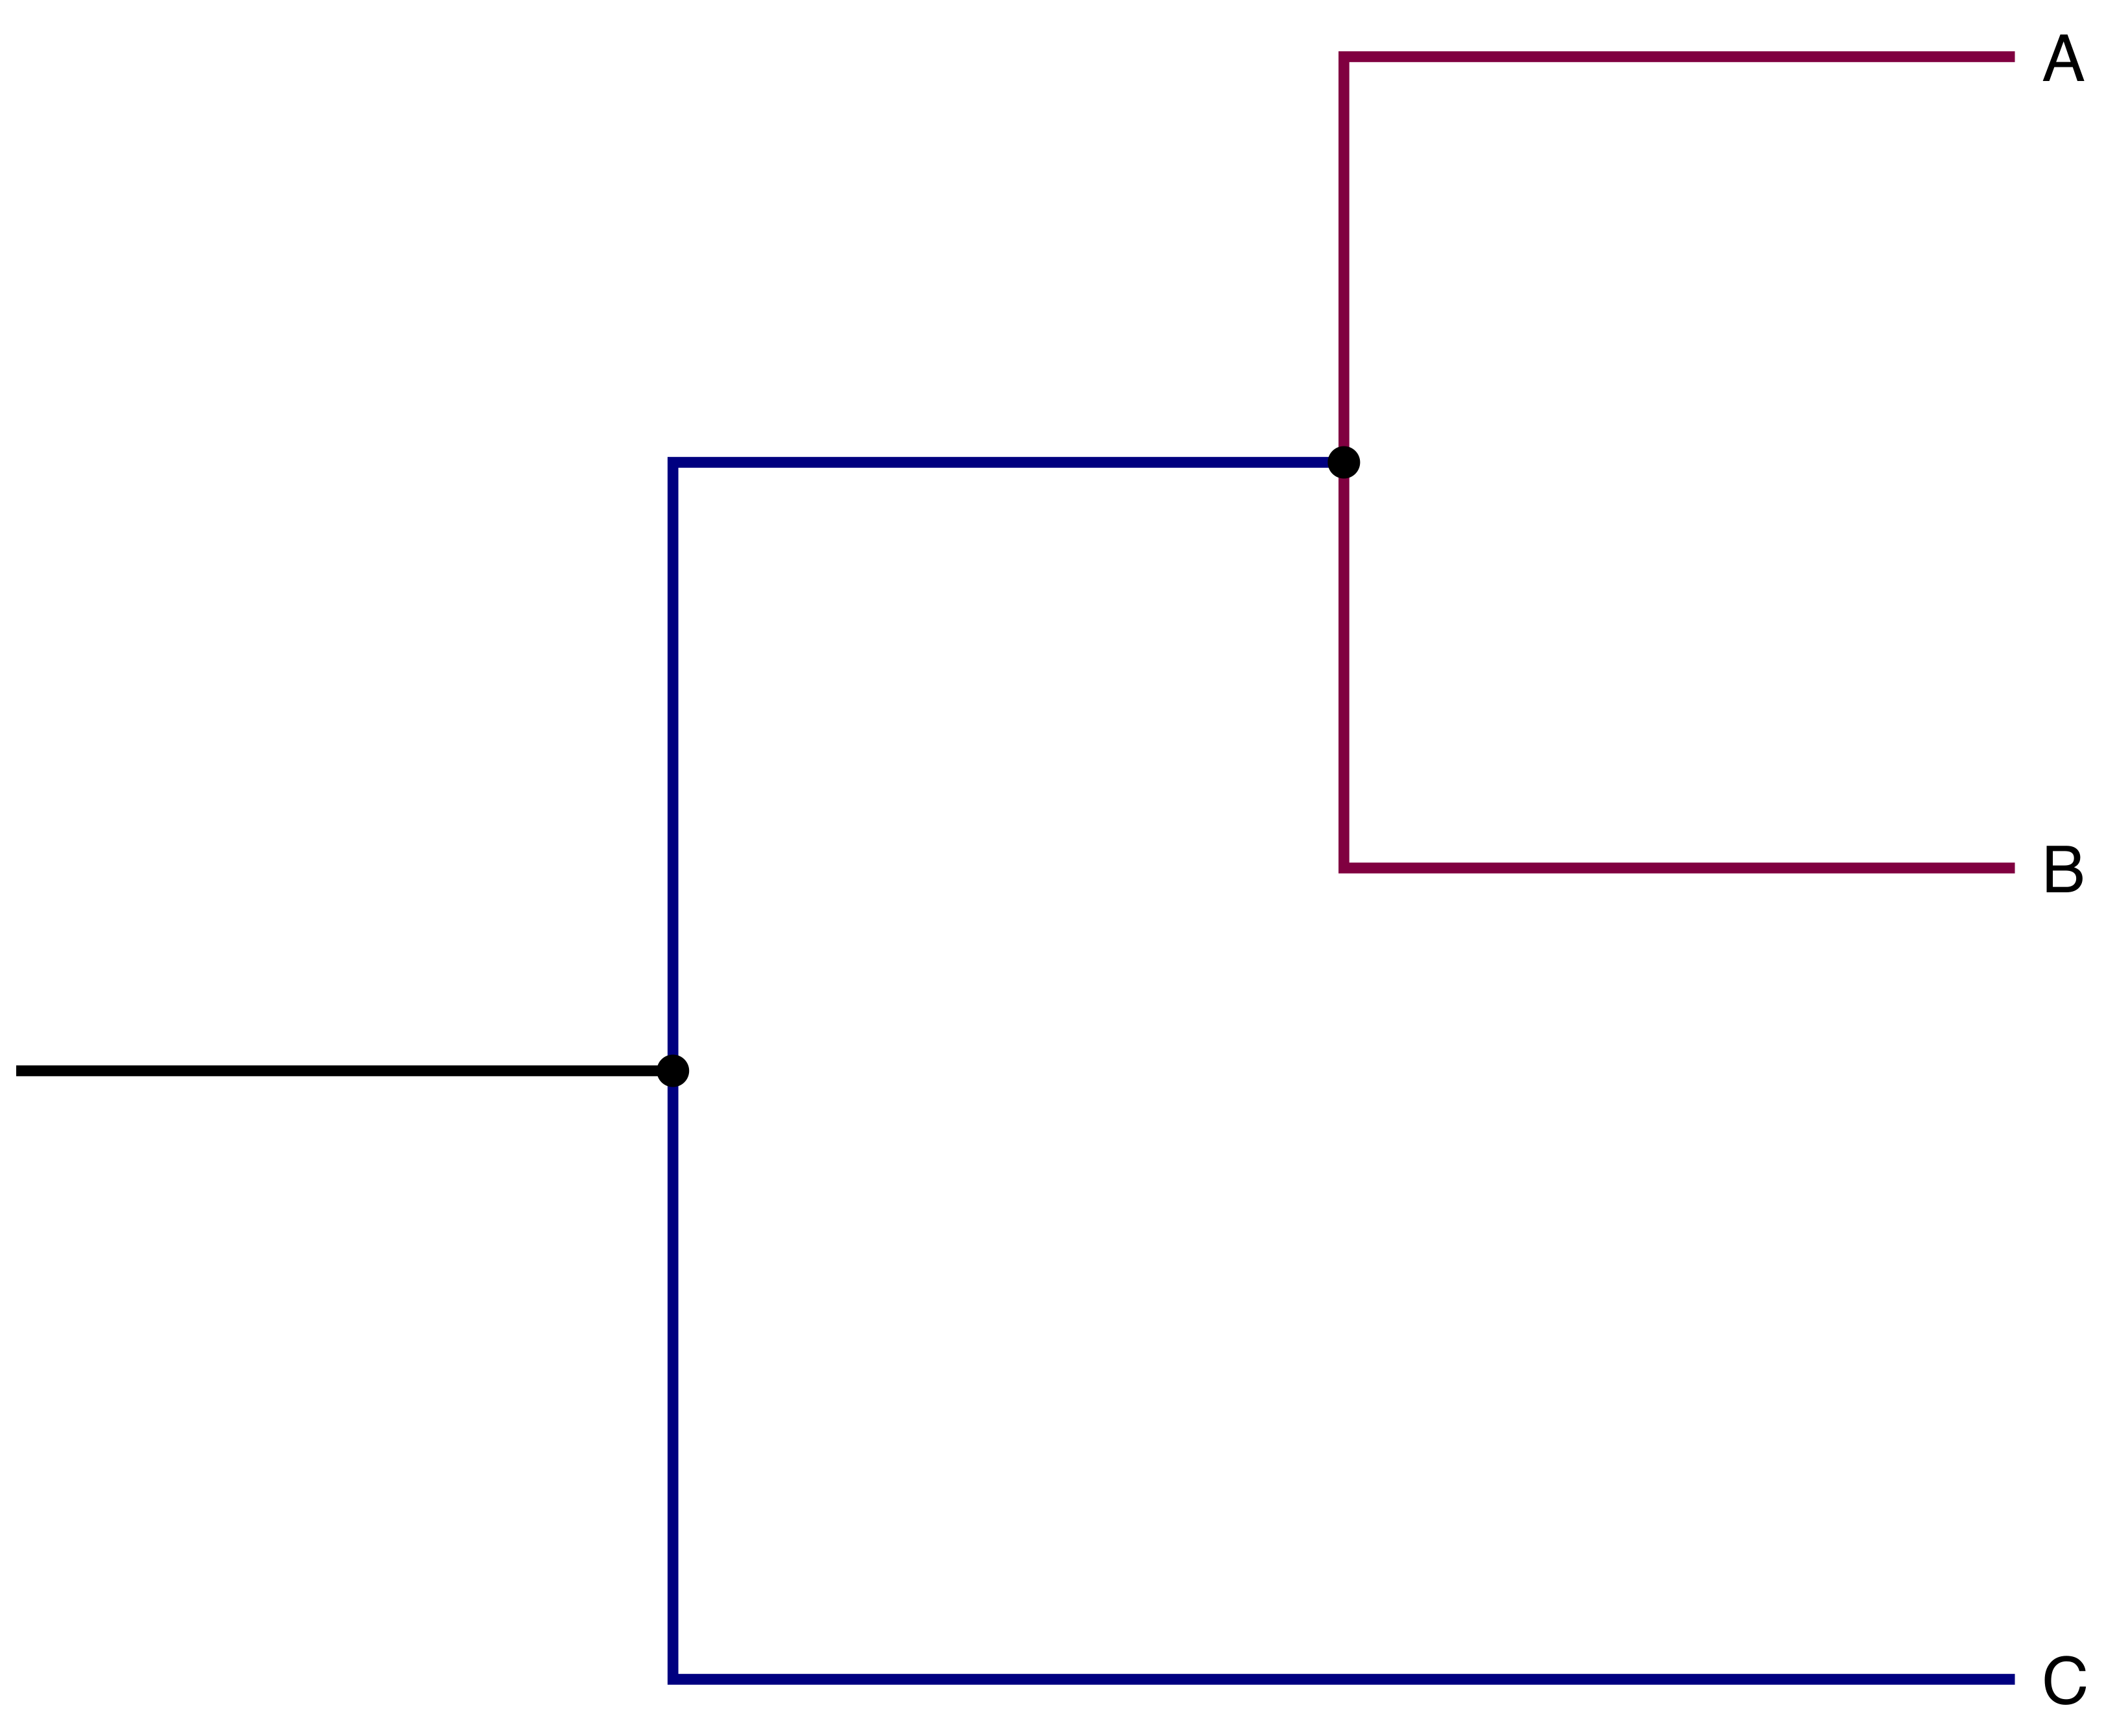
\includegraphics[width=0.5\linewidth]{{figures/phylo.png}}
\centering
\caption[Example of a population history]{
The relationships between populations A, B and C are depicted.
Note how branches of the same color can be simulated in parallel if there is no migration.
}
\label{fig:pop_hist}
\end{figure}

To parallelize the simulations, we need to
(i) simulate each branch of the tree independently and
(ii) put together the bits that are simulated independently at the end.
There are many ways to parallelize the simulations, but see \citet{rodrigues_vignette_2021} for an idea.
Below, I will describe the operation for putting together two (or more) tree sequences,
which has been implemented in \tskit (see \url{https://tskit.dev/tskit/docs/stable/python-api.html#tskit.TreeSequence.union} for the documentation).

The information underlying a tree sequence is stored as a collection of tables which define different features.
This simple tabular format allows for rapid accessing of information.
The main components are the Node, Edge, Site and Mutation tables.
A haploid genome can be thought of as a node in a tree, which exists at a particular time.
An edge defines genetic inheritance between two nodes, and it consists of a parent node, a child node, and the left and right coordinates (along a chromosome) over which the child genome inherited from the parent genome.
A site is a location in the genome, and a mutation defines a change of state at a particular node.
See \lcref{fig:example_ts} for an example tree sequence and \lcref{fig:table_collection} for the corresponding collection of tables.
Note how information about the trees are completely independent from the notion of genetic variation (defined by the Site and Mutation tables).

\begin{figure}[htp]
\centering
\begin{subfigure}[b]{.45\linewidth}
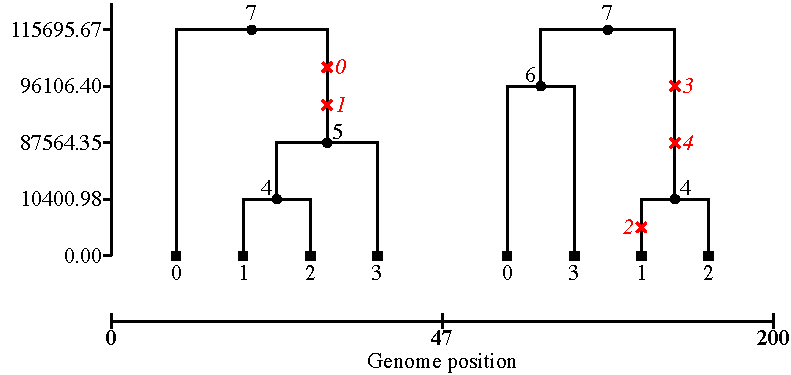
\includegraphics[width=\linewidth]{{union_example/example_ts.pdf}}
\caption{An example tree sequence.}\label{fig:example_ts}
\end{subfigure}
\begin{subfigure}[b]{.45\linewidth}
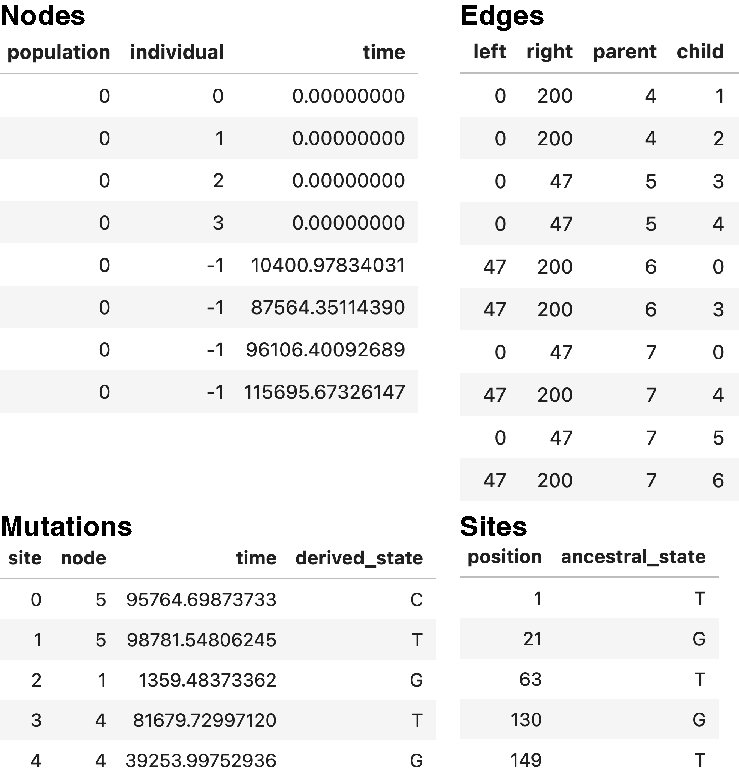
\includegraphics[width=\linewidth]{{union_example/tables.pdf}}
\caption{The underlying collection of tables.}\label{fig:table_collection}
\end{subfigure}
\caption[An example tree sequence and its tabular encoding]{
The relationship between four samples are depicted in a sequence of trees.
Note how because of shared ancestry,
mutations that are common to many of the samples need to be represented only once.
However, in a matrix of variant sites against samples, these mutations would be repeated unnecessarily.
}
\label{fig:example_ts_and_tc}
\end{figure}


After simulating two independent populations,
one might want to obtain the node-wise union of these two tree sequences (\eg for analyzing patterns of between population variation).
This is almost as simple as concatenating the Node, Edge, Site and Mutation tables.
However, nodes from the second tree sequence need to be re-enumerated, and this new numeric order needs to be propagated onto the other tables.
I simulated the history of two populations independently using \msprime \citep{kelleher_efficient_2016, baumdicker_efficient_2022} \plcref{fig:ts1,fig:ts2}.
Then, I used the union operation to merge the two tree sequences \plcref{fig:tsu}.
Lastly, I added the pre-split history to the merged tree sequence so that all samples coalesce back-in-time \plcref{fig:tsu_recap}.
See the code in Python to reproduce this analysis \plcref{code:union}.
By doing the simulation this way, we are able to run the simulation of each extant population in parallel.
In the case of large simulations (as we will see in \lcref{chapter:greatapes}),
this is essential so that we can distribute the memory usage over different computer nodes.

\begin{lstlisting}[language=Python, caption={Python code to union two independently simulated populations using \msprime and \tskit.}, label=code:union, breaklines=true]
import msprime
import numpy as np
import tskit

# First, we build an msprime.Demography object with our two-population history that splits 100,000 units of time ago
demography = msprime.Demography()
demography.add_population(name=``A'', initial_size=10_000)
demography.add_population(name=``B'', initial_size=100)
demography.add_population(name=``C'', initial_size=100_000)
demography.add_population_split(time=100_000, derived=[``A'', ``B''], ancestral=``C'')

# Now, we can simulate the histories of the two extant populations independently
ts1 = msprime.sim_ancestry(samples={``A'':4}, ploidy=1, demography=demography, sequence_length=50, recombination_rate=1e-6, random_seed=123)
ts2 = msprime.sim_ancestry(samples={``B'':4}, ploidy=1, demography=demography, sequence_length=50, recombination_rate=1e-6, random_seed=1)

# Then, we can union these two tree sequences.
# Note that because the two populations do not share any history,
# we specify a `node_mapping' in which none of the nodes in `ts2' have an equivalent in `ts1'.
tsu = ts1.union(ts2, node_mapping=np.full(ts2.num_nodes, tskit.NULL), add_populations=False)

# Finally, we can add the pre-split history to the union'ed tree sequence with msprime.sim_ancestry.
tsu_recap = msprime.sim_ancestry(initial_state = tsu, demography=demography, random_seed=3)
\end{lstlisting}

\begin{figure}
\centering
\begin{minipage}{0.45\textwidth}%
\begin{subfigure}[b]{\linewidth}
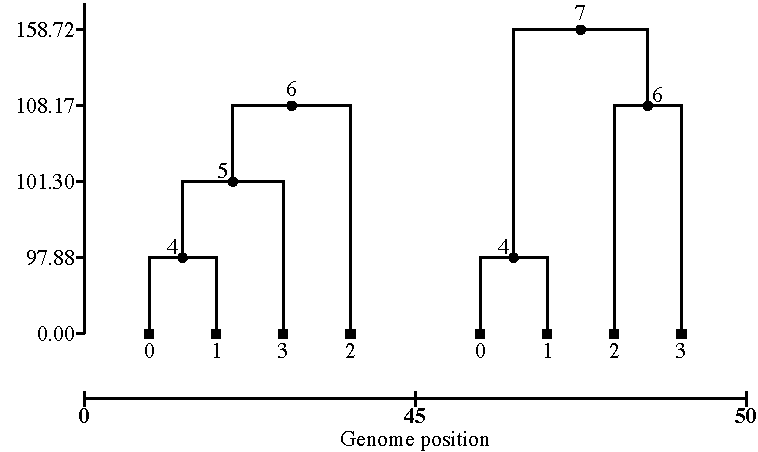
\includegraphics[width=\linewidth]{union_example/ts2.pdf}
\caption{Tree sequence of population 1.}\label{fig:ts1}
\end{subfigure}
\end{minipage}
\begin{minipage}{0.45\textwidth}%
\begin{subfigure}[b]{\linewidth}
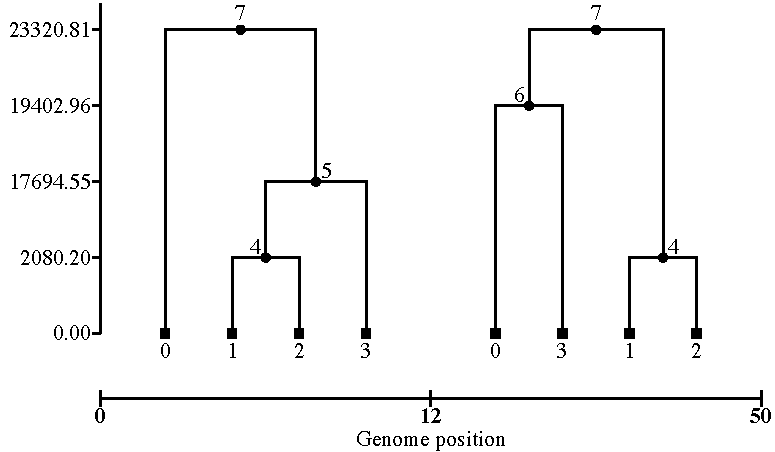
\includegraphics[width=\linewidth]{union_example/ts1.pdf}
\caption{Tree sequence of population 2.}\label{fig:ts2}
\end{subfigure}
\end{minipage}

\begin{subfigure}[b]{.9\textwidth}
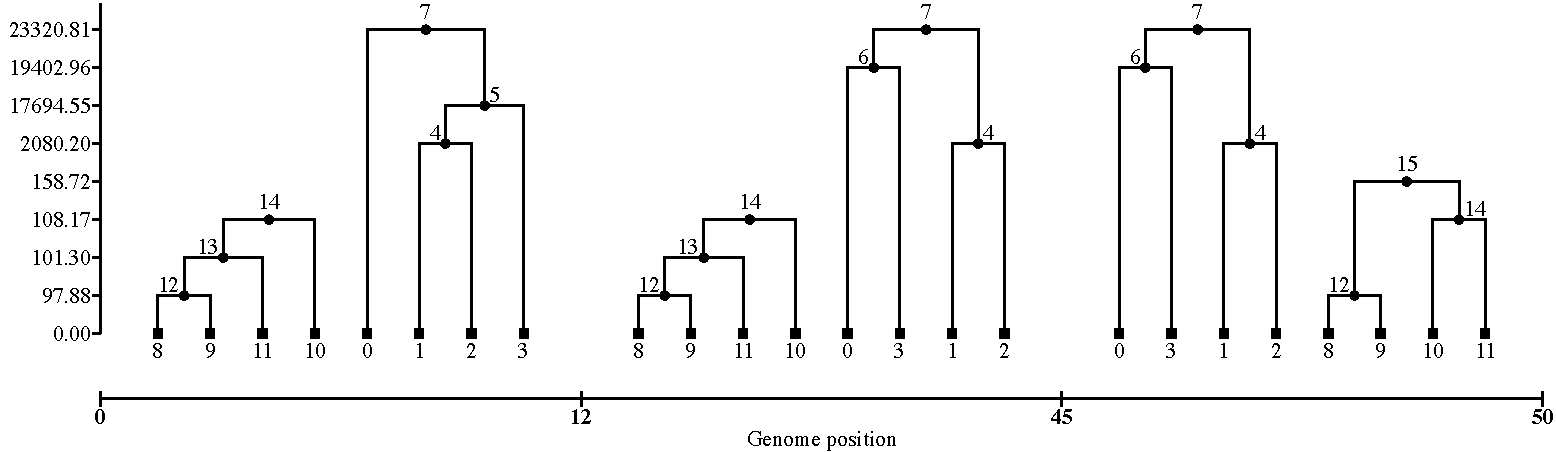
\includegraphics[width=\linewidth]{union_example/tsu.pdf}
\caption{Union of tree sequences 1 and 2.}\label{fig:tsu}
\end{subfigure}

\begin{subfigure}[b]{0.9\textwidth}
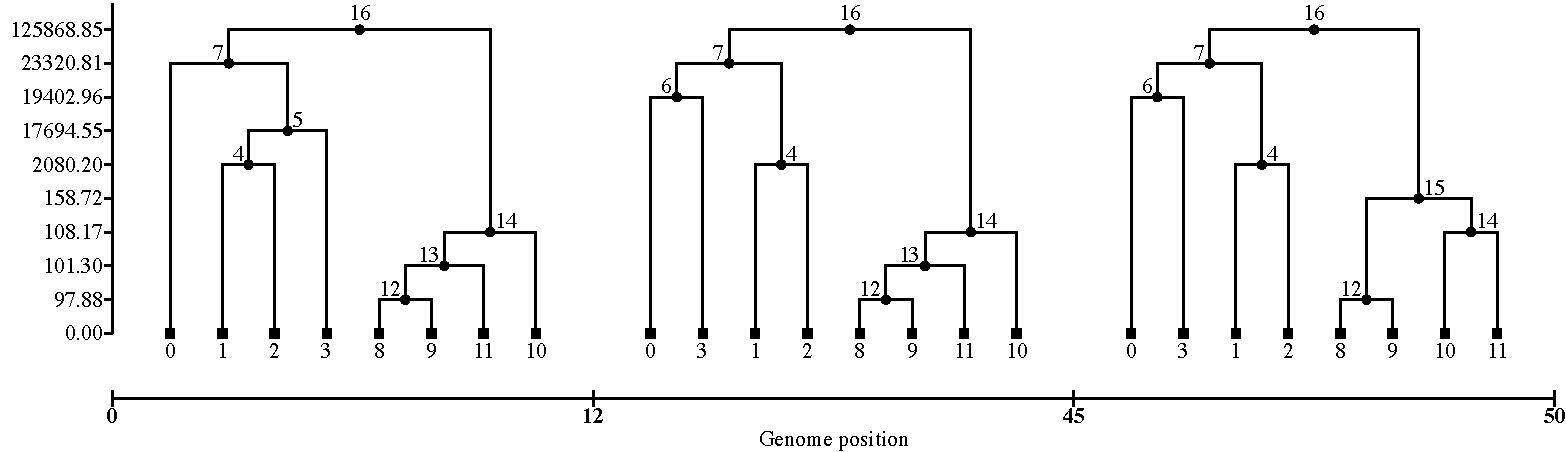
\includegraphics[width=\linewidth]{union_example/tsu_recap.pdf}
\caption{Adding the pre-split history to the union.}\label{fig:tsu_recap}
\end{subfigure}

\caption[The union operation for tree sequences]{The union operation for tree sequences.
(a) and (b) show the tree sequences for two independently simulated populations.
(c) depicts the union of these tree sequences.
(d) shows the merged tree sequences with added history for the ancestral population.}
\label{fig:union_op}
\end{figure}

A trickier use case for the node-wise union operation is when there are two tree sequences which share part of their histories.
That is, imagine you simulate the ancestor population of A and B, and then start two new independent simulations of A and B.
In this case, it is necessary to defined which portions are not shared between the two tree sequences,
so that the histories can be joined properly.
To define the non-shared portions, it is necessary to specify which nodes in one tree sequence are equivalent to those in the other.
Then, the portions that are not shared from one tree sequence are copied over onto the other.
New nodes are given a new numeric identifier which are propagated to the other tables.
Refer to \citet{rodrigues_vignette_2021} for a concrete example on how to union tree sequences with some shared history.

\section{Towards more realistic and reproducible simulations: Introducing models of selection to Stdpopsim}


\newpage
\section{Bridge}

In Chapter II, I presented my contributions to make evolutionary tools more robust and efficient.
To gain insights into the complex interactions between evolutionary processes that shape genetic variation, 
it is necessary to increase the biological realism of our models.
This increase in realism comes at a cost: simulations that are closer to reality take longer to run and consume more computational resources.
In Chapter III, we apply our ideas presented in this chapter on how to parallelize multi-population simulations and on simulating realistic chromosomes.
The realistic simulations we produce in Chapter III were extremely costly, despite our best efforts to optimize, and each replicate took over 30 days to run consuming at the peak over 160Gb of RAM.
Nevertheless, we were able to push the boundaries in what is possible with our tools and computational resources today to answer a long-standing question in evolutionary genetics: What are the relative contributions of different evolutionary processes in shaping genetic variation in the great apes?

\chapter{Shared evolutionary processes shape landscapes of genomic variation in the great apes} \label{chapter:greatapes}

\bigskip
This chapter was published in the journal \emph{Genetics} in 2024. 
Andrew D. Kern and Peter L. Ralph are co-authors on this paper.
Co-authors and I conceptualized the study,
I curated the dataset,
I performed analyses and simulations with input from my co-authors, and
I wrote the manuscript with editorial assistance from my co-authors.

\bigskip
The citation for this publication is as follows:

\fullcite{rodrigues_shared_2024}
\bigskip

\section{Introduction}
% TOPIC: We do not know how much of genetic diversity is determined by positive and negative selection and how does the influence of selection compare to other processes.

Genetic variation is determined by the combined action of mutation, demographic processes, recombination and natural selection.
However, there is still no consensus on the relative contributions of these processes and 
their interactions in shaping patterns of genetic variation.
Two major open questions are: how does the influence of selection compare to other processes?
And, to what degree is genetic variation influenced by beneficial versus deleterious mutations?

Genetic variation can be measured within a species or between species with two related metrics: within-species genetic diversity and between-species genetic divergence.
Both can be estimated with genetic data by computing the per site average number of differences between pairs of samples within a species or between two species.
and these are estimates of the mean time to coalescence.
(Note that we do not discuss \emph{relative divergence},
which is often measured using $F_{ST}$.)
Evolutionary processes impact diversity and divergence in different ways, so the relationship between these carries information regarding these processes.

% TOPIC: How does selection impact diversity?
Natural selection directly impacts genetic diversity because it can reduce the frequencies of alleles that are deleterious (negative selection)
or increase those of beneficial alleles (positive selection).
Selection can also directly affect between-species genetic divergence.
Deleterious alleles are more likely to be lost from the population, thus reducing divergence at the affected sites.
On the other hand, beneficial alleles have a higher probability of fixation.
This leads to an increase in the rate of substitution at sites under positive selection that in turn
increases divergence between species.
Thus, contrasting patterns of diversity and divergence at the same time can help disentangle between modes of selection \parencite{hudson_test_1987}.
Indeed, perhaps the most widely used test for detecting adaptive evolution, the McDonald-Kreitman test,
compares diversity and divergence contrasted between neutral (\eg synonymous) and functional (\eg non-synonymous) site classes \parencite{mcdonald_adaptive_1991}.
This test and its extensions have been applied to a myriad of taxa,
and it has become clear that a substantial proportion of amino acid substitutions
are driven by positive selection in a number of taxa \parencite{smith_adaptive_2002, ingvarsson_natural_2010, slotte_impact_2014,galtier_adaptive_2016}.

Selection also disturbs genetic variation at nearby locations on the genome,
and this indirect effect of selection on diversity is called ``linked selection''.
Linked selection can be caused by at least two familiar mechanisms: genetic hitchhiking and background selection.
Under genetic hitchhiking, as a beneficial mutation quickly increases in frequency in a population,
its nearby genetic background is carried along, causing local reductions in levels of genetic diversity. 
The size of the region affected by the sweep depends on the strength of selection, which determines how fast fixation happens,
and the crossover rate, because recombination allows linked sites to escape from the haplotype carrying the beneficial mutation \parencite{maynard_smith_hitch-hiking_1974,kaplan_hitchhiking_1989}.
Under background selection, neutral variation linked to deleterious mutations is removed from the population
unless, as before, focal lineages escape via recombination \parencite{charlesworth_effect_1993}.
Both of these processes leave similar footprints on patterns of within-species genetic diversity,
and so attempts to determine the contributions of positive and negative selection in 
shaping levels of genetic variation genome-wide have proven to be difficult \parencite{kim_joint_2000, andolfatto_adaptive_2001},
although the processes seem separable more locally \parencite{schrider_soft_2017,schrider_background_2020}.
Importantly, linked selection has more limited effects on between-species genetic divergence,
as a beneficial or deleterious mutation does not affect the substitution rate of linked, neutral mutations \citep{birky_effects_1988}.



% TOPIC: What do we know by effects of selection and what are our limitations? 
The effects of linked selection in shaping genetic variation are pervasive across genomes \citep{begun_levels_1992, cai_pervasive_2009, murphy_broad-scale_2022, lohmueller_natural_2011, corbett-detig_natural_2015, murphy_broad-scale_2022}.
For example, dips in nucleotide diversity surrounding functional substitutions have been uncovered in many taxa, 
such as fruit flies \citep{kern_genomic_2002,sattath_pervasive_2011}, rodents \citep{halligan_contributions_2013}, \textit{Capsella} \citep{williamson_evidence_2014} and maize \citep{beissinger_recent_2016}.
In \textit{Drosophila melanogaster}, levels of synonymous diversity (which is putatively neutral) and amino acid divergence are negatively correlated \citep{andolfatto_hitchhiking_2007, macpherson_genomewide_2007};
positive selection can cause such a pattern if beneficial amino acid mutations are fixing and as they do reducing levels of linked neutral variation via selective sweeps.
In contrast in humans, levels of synonymous diversity are roughly the same near amino acid substitutions and synonymous substitutions,
suggesting recent, recent fixations at amino acids sites may not be the result of strongly beneficial alleles \parencite{hernandez_classic_2011,lohmueller_natural_2011}.
However, in the human genome, amino acid substitutions tend to be located in regions of lower constraint than synonymous substitutions,
implying that the signal of positive selection may be confounded by the effects of background selection \parencite{enard_genome-wide_2014}.
%This example only highlights an overacing difficulty in inferring selection in the presence of linkage.

% TOPIC: Demography complicates inference even further; infeasibility of mathematical models
% TODO: change this to be about simulating positive and negative selection at the same time across multiple sites?
%Inference of the role of selection in shaping genetic variation is complicated further by demography.
%Demographic events can create spurious signatures of selection and erase or amplify true footprints.
%For instance, bottlenecks seem to have exacerbated the reduction of genetic diversity due to background selection in both maize and humans \parencite{torres_human_2018, beissinger_recent_2016}.
%These interactions between selection and demography are difficult to model.
%Recent computational advances have made it possible for us to move from simpler backwards-in-time coalescent models \citep{hudson_testing_1983}
%to more complex and computationally demanding forward-in-time simulations,
%and these have provided a route to studying these hard to model interactions between evolutionary processes \parencite{haller_slim_2019, kelleher_efficient_2016, haller_tree-sequence_2019}.
%With forward-in-time simulations, it is possible to build complex models with many sites under selection and demography.
%Nevertheless, the problem of identifying features of the data that are informative of the strength and mode of selection still remains.

% TOPIC: Modelling interactions between types of selection and other processes
Two major challenges remain in the way of a fuller characterization of the effects of selection on genetic variation:
(i) it is hard to model interactions between evolutionary processes (\eg sweeps within highly constrained regions), and 
(ii) model identifiability is challenging for some summaries of the data (\eg sweeps and background selection may impact diversity in similar ways).
Recent computational advances have made it possible for us to move from simpler backwards-in-time coalescent models \citep{hudson_testing_1983}
to more complex and computationally demanding forward-in-time simulations,
and these have provided a route to studying these hard to model interactions between evolutionary processes across multiple sites \parencite{haller_slim_2019, kelleher_efficient_2016, haller_tree-sequence_2019}.
Simulation-based inference can then allow us to better describe the roles of different modes of selection and other processes in shaping genomic variation.
However, the problem of identifying features of the data that are informative of the strength and mode of selection still remains.

% TOPIC: 
%Large scale patterns of correlation in landscapes of diversity and divergence among related groups of taxa (Stankowski, Buri:W)
One promising approach might be to compare patterns of genetic variation in multiple species jointly
as each species can be thought of as semi-independent realizations of the same evolutionary processes \citep[c.f.][]{won_divergence_2005}.
In speciation genomics studies, it is common to visualize large scale patterns of genetic variation along chromosomes (so-called landscapes of diversity and divergence),
which may contain substantial information to help us disentangle evolutionary processes.
Earlier empirical surveys have focused on the identification of regions of 
accentuated relative divergence between populations \parencite{cruickshank_reanalysis_2014, harr_genomic_2006, turner_genomic_2005},
although patches of increased divergence can be the result of myriad forces besides reproductive isolation and adaptation.
Recent comparative studies have found that landscapes of diversity are highly correlated between related groups of species,
such as \textit{Ficedula} flycatchers \citep{burri_linked_2015, ellegren_genomic_2012}, warblers \citep{irwin_recurrent_2016}, stonechats \citep{doren_correlated_2017}, hummingbirds \citep{battey_evidence_2020}, monkeyflowers \citep{stankowski_widespread_2019}  and \textit{Populus} \citep{wang_evidence_2020}.
\citet{burri_interpreting_2017} proposed that we could capitalize on correlated genomic landscapes to study the interplay between different forms of selection and other evolutionary processes.
Neutral processes, such as incomplete lineage sorting or migration, could potentially produce significant correlations in levels of diversity across species,
however strong correlations have been observed among taxa with long divergence times and without evidence of gene flow. 
For example, \citet{stankowski_widespread_2019} found that landscapes of diversity and divergence are highly correlated across a radiation of monkeyflowers which spans one million year (or about $10N_e$ generations, where $N_e$ is the effective population size),
far longer than what is relevant for incomplete lineage sorting (\ie the coalescent timescale spans just a few multiples of $N_e$).
However, a shared process that independently occurs in the branches of a group of species could maintain correlations over long timescales.
For example, if two species' physical arrangement of functional elements and local recombination rates are similar,
the direct and indirect effects of selection could make it so that peaks and valleys on the landscape of diversity are similar,
maintaining correlation between their landscapes over evolutionary time \parencite{burri_interpreting_2017, delmore_comparative_2018}.
Further, if mutational processes are heterogeneous across the genome in a manner that is shared among species,
then correlated landscapes of diversity could be created through mutational variation as well. 

% TOPIC: Here, we use the great apes as a model to understand what causes correlated landscapes and to tease apart the relative roles of positive and negative selection and other processes such as ancestral variation, mutation rate variation, etc.

Here, we aim to (i) describe whether and in what ways landscapes of within-species diversity and between-species divergence are correlated,
and (ii) to tease apart the relative roles of positive and negative selection and other processes (\eg ancestral variation, mutation rate variation) in shaping patterns of genetic variation.
To understand processes driving these correlations, we employ highly realistic, chromosome-scale, forward-in-time simulations,
since analytical predictions are not available.
We use the great apes as a system to investigate correlated patterns of genetic variation because
there is high quality population genomic data for all species \parencite{prado-martinez_great_2013},
the clade is about 12 million years old or $60 N_e$ generations (but there have not been many chromosomal arrangements \parencite{jauch_reconstruction_1992}),
and lastly the landscapes of gene density, recombination rate and mutation rate are roughly conserved \parencite{kronenberg_high-resolution_2018,stevison_time_2016}.
Our study demonstrates that correlated landscapes can be useful in distinguishing between modes of selection and the balance of direct and linked selection shaping genomic variation.

\section{Methods} \label{sec:methods}

\subsection{Genomic data}

We retrieved SNP calls for ten great ape populations made on high coverage (${\sim}25\times$) short-read sequencing data from the Great Ape Genome Project \citep{prado-martinez_great_2013},
mapped onto the human reference genome (NCBI36/hg18).
We analyzed 86 individuals divided into the following populations: 
human ($n=9$ samples), bonobo ($n=13$), Nigeria-Cameroon chimpanzee ($n=10$), eastern chimpanzee ($n=6$), central chimpanzee ($n=4$), western chimpanzee ($n=4$), eastern lowland gorilla ($n=3$), western gorilla ($n=27$), Sumatran orangutan ($n=5$), Bornean orangutan ($n=5$) (we excluded two samples from the original dataset: the Cross River gorilla and the chimpanzee hybrid).
\citet{prado-martinez_great_2013} applied several quality filters to the SNP calls (see Section 2.1 of their Supplementary Information) and, 
for each species, identified the genomic regions in which it would be unreliable to call SNPs (uncallable regions).
For our downstream analyses, we only considered sites which were callable in all populations.

We calculated nucleotide diversity and divergence ($d_{XY}$) in non-overlapping 1Mb windows using \allel \citep{miles_cgghscikit-allel_2020}.
Windows in which there were less than 40\% callable sites were not used in any of the analyses.
For example, this yielded 129 (out of 132) 1Mb windows in chromosome 12 in which 75\% of the sites were callable on average.

To tease apart the effects of GC-biased gene conversion (gBGC),
we decomposed diversity and divergence by allelic states.
gBGC is expected to affect weak bases (A or T) which are disfavored when in heterozygotes which also carry a strong base (G or C).
Thus, one way understand the effects of gBGC is by comparing sites which were weak to those that were strong in the ancestor (ancestrally strong alleles are not affected by gBGC, but ancestrally weak alleles can be).
We assumed that the state in the ancestor of the great apes to be the state seen in rhesus macaques (genome version RheMac2) --- sites without enough information in RheMac2 were excluded.
Then, we computed divergence only considering sites which were ancestrally weak or ancestrally strong \plcref{fig:anc-partitioned_dxy}.
This approach has two major drawbacks: (i) many of the sites cannot be used because they are missing in RheMac2 and (ii) sites can be mispolarized.
Thus, we came up with a second approach to tease apart the effects of gBGC on correlations between genomic landscapes.
When comparing two landscapes of divergence (which encompass four species),
we can classify each site by the change in state that happened without needing to polarize mutations by looking at the ancestor.
For example, if we have allelic states for four species and we see A-A-T-T as the configuration of alleles at a particular site,
we know that there must have been one mutation which changed the state from a weak base to another weak base (W-W).
On the other hand, if we see A-G-A-A there must have been one mutation from weak to strong (W-S) (or vice-versa).
Sites with multiple mutations (\eg A-G-G-C) were removed from the analyses.
Sites that did not change from W to S (or vice-versa) are not expected to be affected by gBGC,
and we refer to these as W-W or S-S mutations \plcref{fig:partitioned_dxy}[A].
Sites where there may have been a weak to strong change (W-S mutations) may be affected by gBGC \plcref{fig:partitioned_dxy}[B].
We only considered windows with at least 5\% of callable sites in these analyses.


\subsection{Simulations}\label{sec:methods:simu}

We implemented forward-in-time Wright-Fisher simulations of the entire evolutionary history of the great apes using \slim \citep{haller_slim_2019, haller_tree-sequence_2019}.
Each branch in the great apes' tree was simulated as a single population with constant size \plcref{fig:sim_demog}.
Population splits occurred in a single generation, 
and there was no contact between populations post-split.
Population sizes and split times were taken from the estimates in \citet{prado-martinez_great_2013}.
Across all our simulations, we simulated crossover events occurred with the sex-averaged rates from the deCODE genetic map (in assembly NCBI36/hg18 coordinates) \citep{kong_high-resolution_2002}.
We then computed diversity and divergence in the same windows used for the real data using \tskit \citep{kelleher_efficient_2018, ralph_efficiently_2020}.

To improve run time, we simulated sister branches in parallel and recorded the final genealogies as tree sequences \citep{kelleher_efficient_2016}.
Further, neutral mutations were not simulated with \slim and were added after the fact with \msprime.
The resulting tree sequences were later joined and recapitated (\ie we simulated genetic variation in the ancestor of all great apes using the coalescent) using \msprime, \tskit and \pyslim \citep{kelleher_efficient_2016, kelleher_efficient_2018, rodrigues_vignette_2021}.
Despite our efforts to improve run time, our simulations of the entire history of the great apes were still incredibly costly (taking over a month to complete in many instances).

In our neutral simulations, we assumed that neutral mutations occurred at a rate of $\expnumber{2}{-8}$ new mutations per generation per site, uniformly across the chromosome.
To understand the effects of natural selection on landscapes, we simulated beneficial and deleterious mutations only within exons,
assuming that the locations of exons were shared across all great apes \citep{kronenberg_high-resolution_2018} and using exon annotations from the human reference genome NCBI36/hg18.
We varied the proportions of neutral, beneficial and deleterious mutations within exons, 
but the distribution of fitness effects for both deleterious and beneficial mutations were shared across all apes.
In total, we explored 26 different parameter combinations with different simulations (see \lcref{tab:sim_space} and \lcref{tab:sim_params} for the parameter space).

To simulate local variation in mutation rates along the chromosome, 
we used the neutral genealogy we simulated with \slim (and recapitated with \msprime) and stripped all existing mutations from it.
Using this genealogy, we added neutral mutations back with varying levels of (neutral) mutation rate variation along the chromosome (using \msprime).
We built mutation rate maps by sampling mutation rates for each 1Mb window independently from a normal distribution with mean $\expnumber{2}{-8}$
and standard deviation chosen from $\frac{\sigma}{\expnumber{2}{-8}} = \{ 0.010, 0.017, 0.028, 0.046, 0.077, 0.129,\allowbreak 0.215, 0.359, 0.599, 1.000 \}$.


\begin{table}[htb]
\caption[Range of parameters explored in the simulations]{Range of parameters explored in the simulations. Non-neutral mutations were only allowed within exons. 
``DFE'' refers to the distribution of fitness effects. 
Gamma distribution was parameterized with shape $\alpha$ and mean $\bar{s}$=$\alpha/\beta$, where $\beta$ is the rate parameter.}
\label{tab:sim_space}
\resizebox{\textwidth}{!}{
\begin{tabular}{@{}lllll@{}}
\toprule
\textbf{Regime}                     & \textbf{Neutral} & \textbf{Deleterious only}                                                                               & \textbf{Beneficial only}                                                                  & \textbf{Both}                                                                                           \\ \midrule
Proportion of deleterious mutations & 0\%              & 10\% -- 70\%                                                                                            & 0\%                                                                                       & 10\% -- 70\%                                                                                            \\
Proportion of beneficial mutations  & 0\%              & 0\%                                                                                                     & 0.005\% -- 0.5\%                                                                          & 0.005\% -- 0.5\%                                                                                        \\
Deleterious DFE                     &   ---               & \begin{tabular}[c]{@{}l@{}}Gamma distributed with \\$\bar{s}=\left\{-0.015,-0.03\right\}$ and $\alpha=0.16$\end{tabular} &                                                      ---                                     & \begin{tabular}[c]{@{}l@{}}Gamma distributed with \\$\bar{s}=\left\{-0.015,-0.03\right\}$ and $\alpha=0.16$\end{tabular} \\
Beneficial DFE                      &           ---       &  ---                                                                                                       & \begin{tabular}[c]{@{}l@{}}Exponentially distributed with \\$\bar{s}=\left\{0.01,0.005\right\}$\end{tabular} & \begin{tabular}[c]{@{}l@{}}Exponentially distributed with \\$\bar{s}=\left\{0.01,0.005\right\}$\end{tabular}            \\ \bottomrule
\end{tabular}}
\end{table}


\begin{figure}[htp]
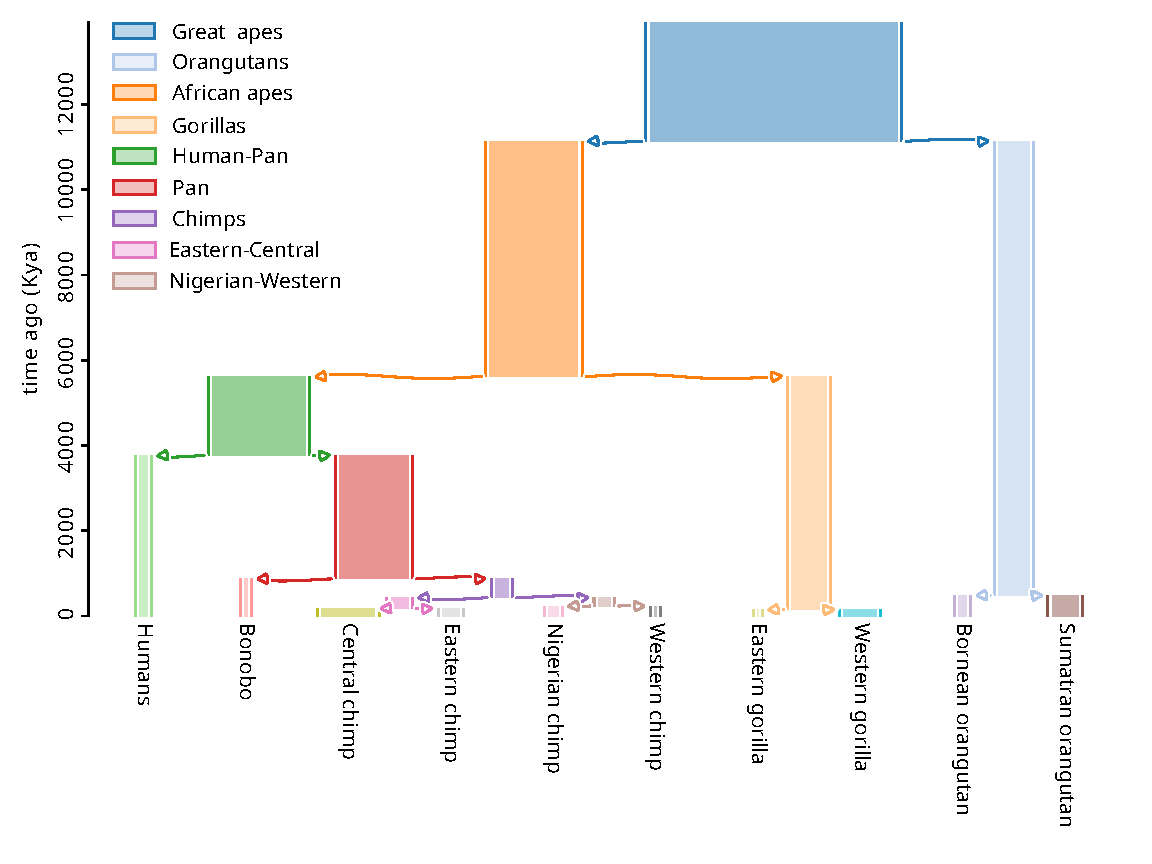
\includegraphics[width=\linewidth]{{figures/demog_tubes_greatapes.pdf}}
\centering
\caption[Simulated demographic history of the great apes]{Range of parameters explored in the simulations. Arrows indicate population splits. Branch widths are proportional to population size. For example, the population size was $125,089$ for the great apes branch and $7,672$ for the humans branch. Figure was produced using \emph{demesdraw} \citep{gower_demes_2022}.}
\label{fig:sim_demog}
\end{figure}

\subsection{Visualizing correlated landscapes of diversity and divergence}\label{sec:methods:visualizing}

To compare landscapes of diversity and divergence along chromosomes, we computed the Spearman correlation between the landscapes across windows within a chromosome.
Because of computational constraints, we focus on chromosome 12.
Chromosome 12 is one of the smallest chromosomes in the great apes, there are no major inversions, and it has good variation in exon density and recombination rate.
The choice was made blindly before looking at the data, but we found it behaves similarly to other chromosomes (see \lcref{fig:chr1_land} through \lcref{fig:chr22_land}).

We expected landscapes of two closely related species to be more correlated than the landscapes of two distantly related species.
Thus, the correlation between any two landscapes of diversity and divergence is expected to depend on distances between them in the phylogenetic tree.
We decided to plot our correlations against distance (in generations) between the most common recent ancestor (MRCA) of each landscape.
In comparing two landscapes of diversity, this amounts to the total distance between the two tips in the species tree.
For instance, the phylogenetic distance $dT$ between diversity in humans and diversity in bonobos is the sum of the lengths of the human, pan and bonobo branches in the species tree \plcref{fig:sim_demog}.
In comparing a landscape of diversity to a landscape of divergence, this amounts to the distance between the species of the landscape of diversity and the MRCA of the two species involved in the divergence.
For example, $dT$ for the landscapes of diversity in humans and divergence between Sumatran orangutans and eastern gorillas would be the distance between the humans tip and the great apes internal node.
$dT$ for the landscapes of divergence between the orangutans and divergence between the gorillas would be the distance between the orangutan and gorilla internal nodes.
Some divergences may share branches in the tree, but these are excluded from our main figures; see \autoref{sec:share} and \lcref{fig:land_cors_bo}.

\section{Results}

First, we will provide a qualitative view of the landscapes of diversity and divergence in the great apes.
Then, we explore the correlations between landscapes in the real data and how they vary depending on phylogenetic distance.
To understand the processes that can drive these correlations, we use forward-in-time simulations of the great apes history under different models (\eg, with and without natural selection).
Lastly, we describe how genomic features are related to patterns of diversity and divergence in the real great apes data,
and we speculate which processes can explain what we see in the data and simulations.


\subsection{Landscapes of within-species diversity and between-species divergence}

% General obs in the landscapes of diversity
There is considerable variation in levels of genetic diversity across the great apes \plcref{fig:chr12_landscapes}.
Species may differ in overall levels of diversity due to population size history: 
species with greater historical population sizes (\eg central chimps and western gorillas) harbor the most amount of genetic variation \citep{prado-martinez_great_2013}.
Levels of diversity vary along the chromosome, but do not appear to be strongly structured.
Instead, diversity seems to haphazardly fluctuate up and down along the chromosome,
and this variation might be attributed to neutral genealogical and mutational processes alone.
A notable feature is the large dip in diversity around the 50Mb mark,
which is so extensive that it almost erases the differences between-species.
This dip coincides with three of the windows with the highest exon density,
possibly pointing to the role of selection in shaping genetic variation in those windows.

% General obs in the landscape of divergence
Levels of between-species genetic divergence also vary along the genome, by an even greater amount in absolute terms.
Interestingly, diversity ($\pi$) varies (along the chromosome) by about $0.2\%$, whereas divergence ($d_{XY}$) varies by more than $0.5\%$.
Because $d_{XY} = \pianc + rT$ (where $\pianc$ is diversity in the ancestor, $r$ is the substitution rate and $T$ is the split time between the two species),
this excess in variance may be due to the substitution process.
Landscapes of divergence which share their most common recent ancestor (\eg human-Bornean orangutan and bonobo-Bornean orangutan divergences --- both colored in red in \lcref{fig:chr12_landscapes}[A]) overlap almost perfectly with each other.
%The diversity dip at 50Kb is not present in the landscapes of divergence, but rather there seem to be increase in divergence,
%a signature that is typically associated with positive selection (decrease in within population variation, but increase in between population divergence).
Curiously, divergence seems to accumulate faster in the ends of the chromosome, leading to a ``smiley'' pattern in the landscape of divergence
--- which is not apparent in the landscape of diversity.
That is, with deeper split times, divergence in the ends of the chromosome seem to increase faster than in other regions of the genome (see how the divergences whose MRCA is the great apes look more like a convex parabola than a horizontal line in \lcref{fig:chr12_landscapes}[A]; see also \lcref{fig:pidxy-change}).
%There is nothing unusual with respect to density of exons in the telomere-proximal regions of this chromosome,
%but crossover rates are higher.
%Crossover and gene conversion rates are correlated in the human genome.
%GC-biased gene conversion, the bias in the mismatch repair of DNA machinery towards guanine or cytosine (GC) alleles,
%can accelerate substitution rates, mimicking one of the hallmarks of positive selection.
%Thus, it is possible that the accumulation of divergence in the telomere-proximal regions is caused by gBGC.

In comparing landscapes across species side by side, 
a remarkable pattern emerges: levels of genetic diversity and divergence along chromosomes have similar peaks and troughs.
To get a sense of how strong this observation is, we can compare it to one of the most well studied properties of genomic variation:
the correlation between exon density and genetic diversity.
We found that the correlation between human diversity and exon density is $-0.2$ (at the 1Mb scale),
but the correlation between levels of diversity in humans and western gorillas is $0.48$.
Below, we dissect this observation of strong correlation between landscapes across the great apes and discuss the processes that may cause it.


\begin{figure}[htp]
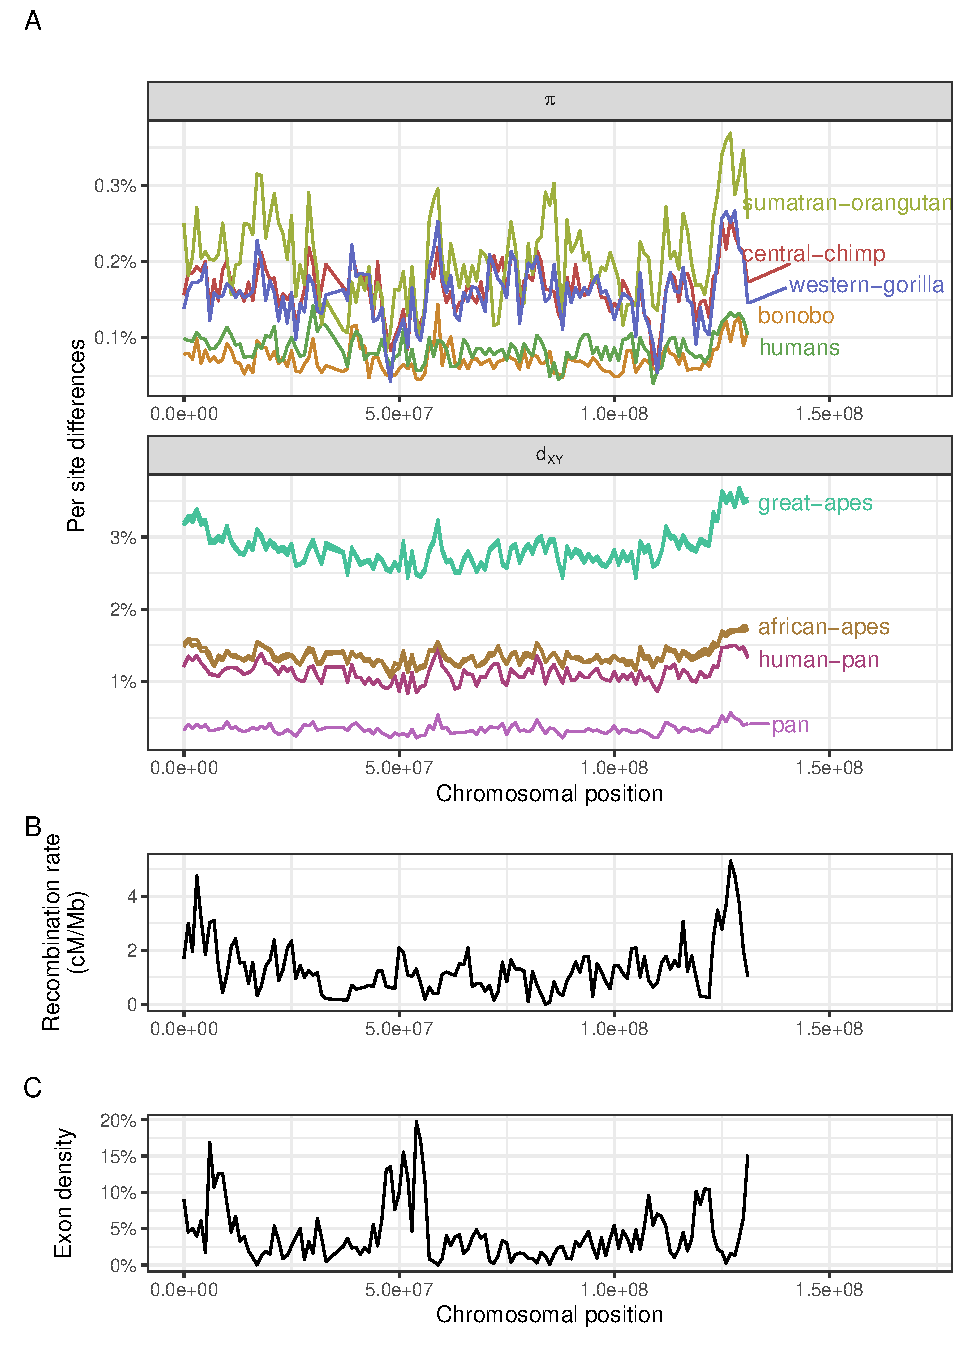
\includegraphics[width=0.8\linewidth]{{figures/chr12-pidxy-landscapes.pdf}}
\centering
\caption[Landscapes of diversity, divergence, recombination rate and exon density]{
A) Landscapes of nucleotide diversity ($\pi$) and divergence ($d_{XY}$) in 1Mb windows along chromosome 12.
Nucleotide diversity and divergence ($d_{XY}$) across 1Mb windows (non-overlapping) of chromosome 12 are displayed above.
Lines are colored by species on the left plot and by the most common recent ancestor (MRCA) on the right.
Genomic windows with less than 40\% of callable sites were masked.
Only a subset of the species are displayed for clarity.
B) Recombination rate estimates from humans (deCODE map; \cite{kong_fine-scale_2010}).
C) Exon density along chromosome 12, computed as the percentage of callable nucleotides in a window that fall within an exon.
}
\label{fig:chr12_landscapes}
\end{figure}

\subsection{Remarkable correlations between landscapes of diversity and divergence}

The landscapes of diversity and divergence are highly correlated across the great apes.
To interpret this signal, we first need to understand what processes can cause such correlations, 
and so first we describe the toy example depicted in \lcref{fig:conceptual_tree}.
Both genetic diversity ($\pi$) and divergence ($d_{XY}$) are estimates of the mean time to the most recent common ancestor (multiplied by twice the effective mutation rate).
Populations \emph{V} and \emph{W} split recently, 
and so samples from one population may coalesce first with a sample from another population (\eg samples $v_2$ and $w_1$),
a pattern called incomplete lineage sorting (ILS).
This causes $\pi_V$ and $\pi_W$ to be correlated with each other, 
as they share some ancestral variation (see the branch marked with \emph{*} in the gene tree).
The probability two samples from \emph{V} coalesce before the split with \emph{W} is $1-e^{\frac{-T}{2N_e}}$,
where $T$ is the split time and $N_e$ is the effective population size.
With longer split times ($T$), we would expect less incomplete lineage sorting; 
therefore, split time ($T$) should be a good predictor of the correlation between two landscapes of diversity (and/or divergence).
Thus, we decided to visualize correlations between landscapes of diversity and divergence by computing the phylogenetic distance $dT$, which is simply the distance in generation time between two statistics.
For example, we define $dT(\pi_W, d_{XY}) = 2T_{VWXY} - T_{XY}$.
Divergences may share branches by definition (irrespective of split times), as you can see with $d_{VX}$ and $d_{XY}$ (see \autoref{sec:methods:visualizing} for more details).
In such cases, our chosen metric $dT$ would not be a good proxy for expected correlations, so we omit such cases from our main figures.
See \autoref{sec:methods:visualizing} and \lcref{fig:land_cors_bo} for more on the correlations between landscapes that share branches.

\begin{figure}[htp]
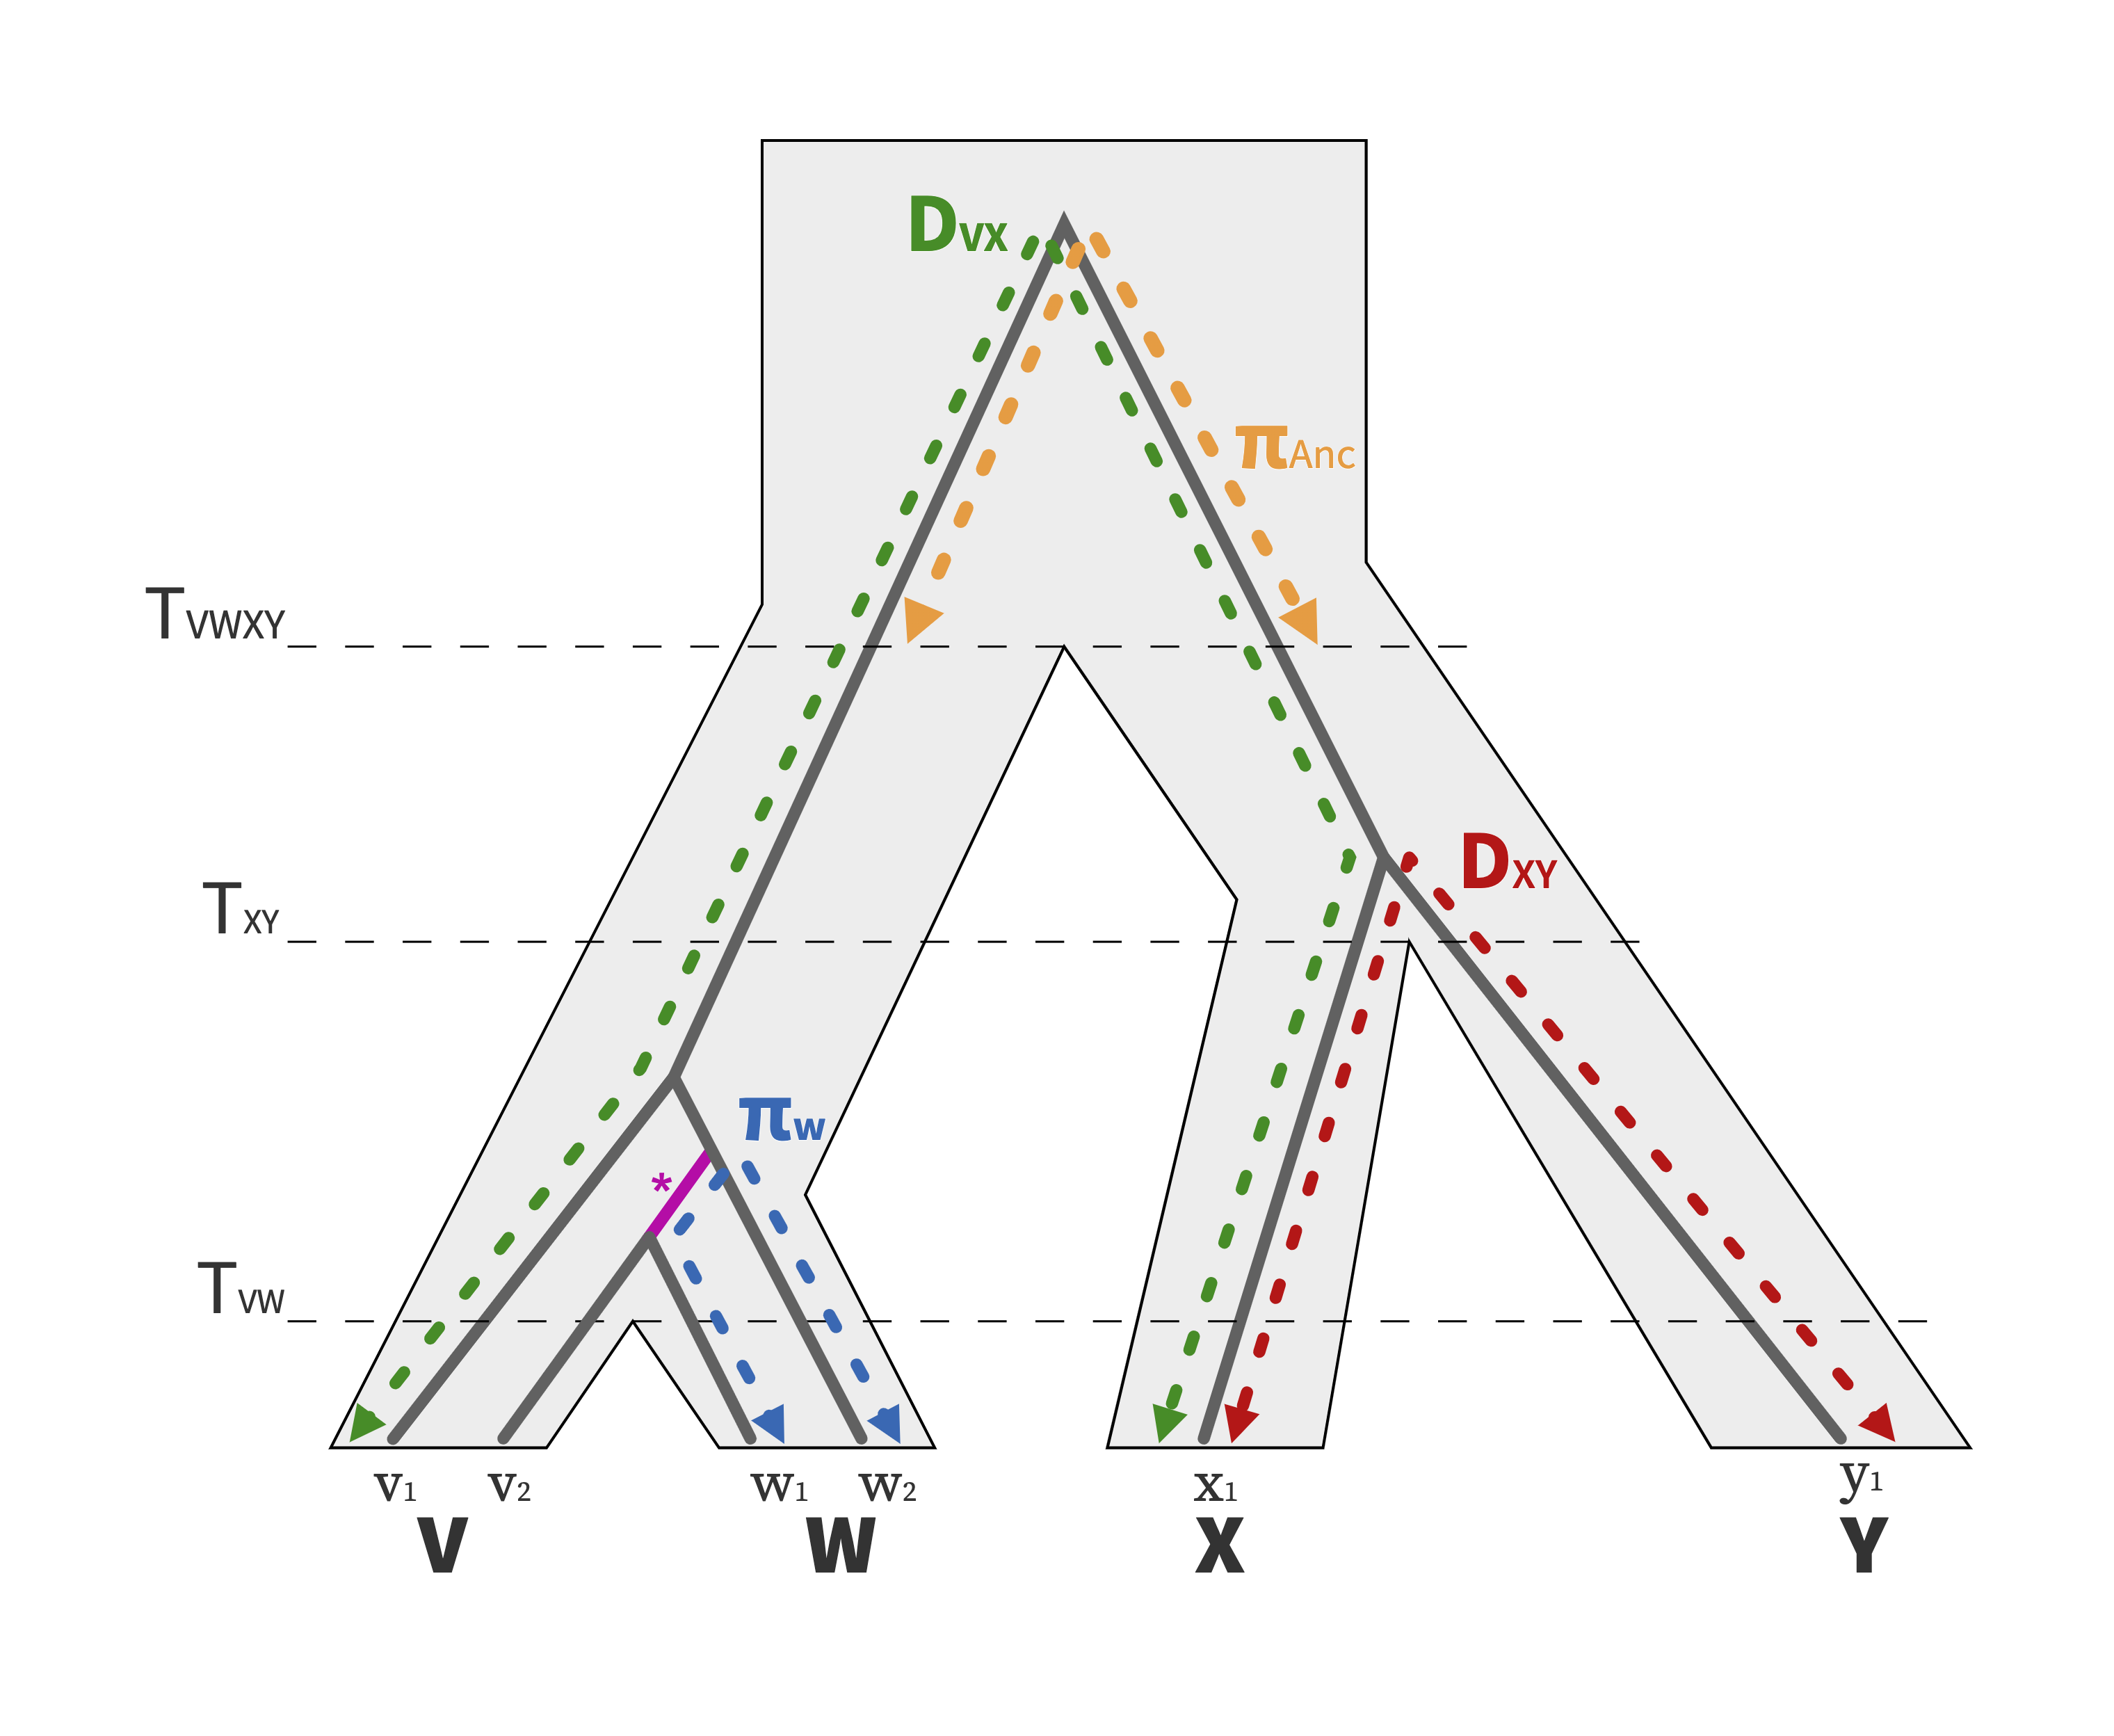
\includegraphics[width=\linewidth]{{figures/conceptual_tree_option2@2x.png}}
\centering
\caption[Visualizing the relationships between nucleotide diversity and divergence statistics between closely related taxa]{Visualizing the relationships between nucleotide diversity and divergence statistics between closely related taxa. 
A population and gene tree for four populations (V, W, X, Y) are depicted with the light gray polygon and gray solid line, respectively.}
\label{fig:conceptual_tree}
\end{figure}

\lcref{fig:land_cors} shows the pairwise correlations between great apes landscapes of diversity and divergence against phylogenetic distance ($dT$).
We see ancestral variation seems to play a role in structuring correlations between landscapes: 
pairs of species that recently split have their landscapes of diversity highly correlated.
Surprisingly, correlations still plateau at around $0.5$.
We expect ancestral variation to play a minor role when comparing orangutans and chimps, which separated around $60 \times N_e$ generations ago,
but their landscapes are still highly correlated.
Population size history seems to affect the correlation between landscapes 
since the weakest correlations involve the landscape of diversity of one of the species with small historical population sizes (\ie bonobos, eastern gorillas and western chimps).


Correlations between landscapes of divergence and diversity and between landscapes of divergence are also quite high, often surpassing $0.5$, 
and they also decay with phylogenetic distance ($dT$) (see middle and right most plots in \lcref{fig:land_cors}).
In theory, these landscapes can also be correlated due to ancestral variation.
To see how ancestral variation can create correlations even between landscapes with no overlap in the tree, consider \lcref{fig:conceptual_tree}:
divergence between X and Y and divergence between V and W can each contain contributions from ancestral diversity if lineages have not coalesced in both branches leading from the ancestor.
If a particular portion of the genome happens to have higher diversity in the ancestor, it will also have higher divergence.
Since this correlation is produced by incomplete lineage sorting, it is expected to have a very small effect except when branches are short.
As discussed in \autoref{sec:methods:visualizing}, two divergences can also be correlated by definition (because they share branches in the tree).
For example, when comparing human-Bornean orangutan and gorilla-Bornean orangutan divergence we expect some correlation because these divergences share the large African apes and orangutan branches in the tree \plcref{fig:sim_demog}.
In \lcref{fig:land_cors} we excluded these comparisons where branches are shared.
Such comparisons can be seen in \lcref{fig:land_cors_bo}.
We found that even these comparisons that share branches have an excess of correlation compared to a theoretical expectation (derived from a simplified neutral model),
that is the correlations are above the $y=x$ line in \lcref{fig:land_cors_bo} even for distantly related species.

There are many processes that could maintain landscapes correlated.
Above, we discussed how we expect ancestral variation to explain these correlations.
The alternative would be to have a process that structures variation along chromosomes which is shared across species.
Using forward-in-time simulations, 
we set out to (i) confirm that ancestral variation alone is not causing landscapes to remain correlated, 
and (ii) test which process or processes that when shared among a group of species could maintain correlations in similar ways to what we observed in the great apes' data. 

\begin{figure}[htp]
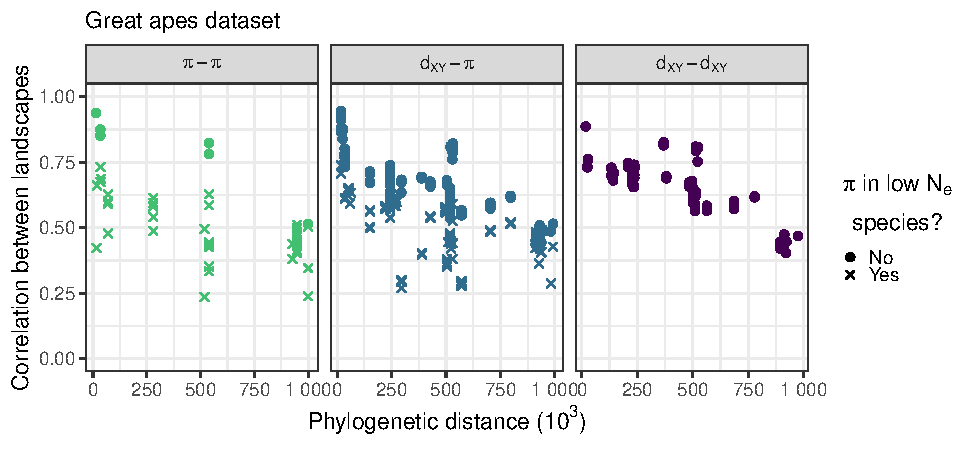
\includegraphics[width=\linewidth]{{figures/cor-pidxy-dT_data.pdf}}
\centering
\caption[Correlations between landscapes of diversity and divergence across the great apes]{
Correlations between landscapes of diversity and divergence across the great apes.
Each point on the plots correspond to the (Spearman) correlation between two landscapes of diversity/divergence, computed on 1Mb windows across the entire chromosome 12. 
Correlations were split by type of landscapes compared ($\pi-\pi$, $\pi-d_{XY}$, $d_{XY}-d_{XY}$). 
$dT$ is the phylogenetic distance (in number of generations) between the most common recent ancestor of the two landscapes compared (\eg the $dT$ for correlation between landscapes of diversity in humans and divergence between eastern gorillas and orangutans is distance between the humans and the great apes nodes in the phylogenetic tree, \lcref{fig:sim_demog}). 
Note that species with low $N_e$ --- for which the estimated species $N_e$ was less than $\expnumber{8}{3}$: bonobos, eastern gorillas and western chimps --- have a different point shape. 
Only comparisons for which the definition of the statistics do not overlap are shown, as explained in \autoref{sec:methods:visualizing}.
}
\label{fig:land_cors}
\end{figure}


\subsection{Neutral demographic processes}

To assess the extent to which ancestral variation alone could explain our observations, 
we performed a forward-in-time simulation of the great apes' evolutionary history.
As expected, the resulting landscapes of diversity and divergence are not well correlated \plcref{fig:neutral_sims}.
Ancestral variation seems to maintain correlations between some landscapes;
for instance, the landscapes of diversity in central and eastern chimps have a $0.61$ correlation, the highest across all pairs of comparisons \plcref{fig:neutral_sims}[A, point \emph{a}].
Nevertheless, correlations between landscapes of diversity and divergence decay quickly with phylogenetic distance to $0$.
Some distant comparisons are moderately correlated
(\eg the landscape of diversity in Bornean orangutans and 
divergence between central and western chimps have a correlation coefficient of $0.23$, see \lcref{fig:neutral_sims}[A, point \emph{b}]),
but that seems to be driven by the outlier window around 80Mb.
This outlier window has a recombination rate close to $0$ \plcref{fig:chr12_landscapes}[C],
so the average nucleotide diversity over the window has a higher variance because of coalescent noise
(see the extreme peaks and valleys in \lcref{fig:neutral_sims}).
Recombination rate variation can create some moderate correlations, 
but when we look at multiple species at once it becomes clear that the mean correlation goes to $0$.

\begin{figure}
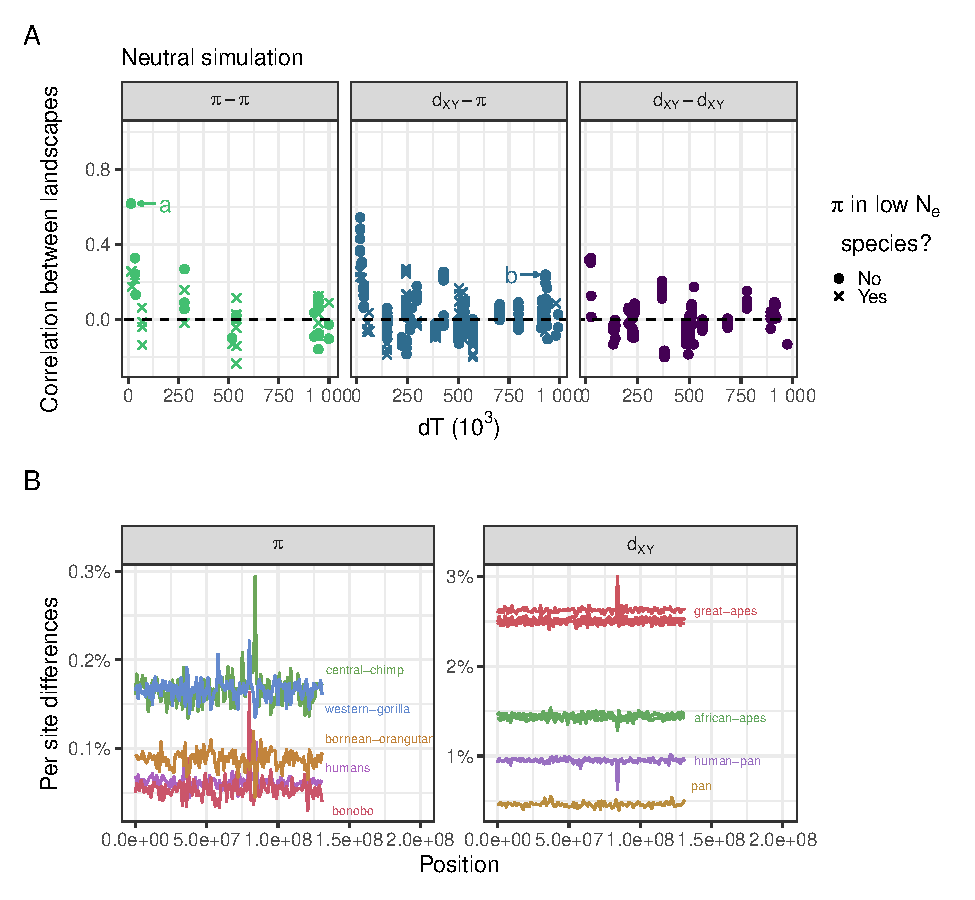
\includegraphics[width=\linewidth]{{figures/corr-pidxy-land-panel_neutral.pdf}}
  \caption[Landscapes are not well correlated in a neutral simulation]{Landscapes are not well correlated in a neutral simulation.
  (A) Correlations between landscapes of diversity and divergence in a neutral simulation. See \lcref{fig:land_cors} for more details.
  (B) Nucleotide diversity and divergence along the simulated neutral chromosome. See \lcref{fig:chr12_landscapes}[A] for details.
}
\label{fig:neutral_sims}
\end{figure}


\subsection{Mutation rate variation}

Since mutation rate can vary along chromosomes,
if this mutation rate map were shared across species,
it would maintain correlations between landscapes over longer periods of time.
To assess this, we used our existing simulated neutral history of the great apes and replaced all mutations
assuming a common mutation rate map across all great apes:
for each window, we drew a mutation rate from a normal distribution with mean $\expnumber{2}{-8}$ (the same as all other simulations) 
and standard deviation $\mu_{\SD}$.
We found that a mutation rate map with $\mu_{\SD}$ close to $8\%\times\expnumber{2}{-8}$ would be needed to get correlations similar to the data \plcref{fig:mutvar_land_cors}[C].
Although mean correlations look similar to the data, we see that correlations tend to increase slightly with time in the simulations with mutation rate variation.
This is expected because windows with higher mutation rate accumulate divergence faster, creating a correlation with mutation rate that gets stronger with time.
In the great apes' data, however, we see a slow but steady decrease in correlations with time.

\begin{figure}[htp]
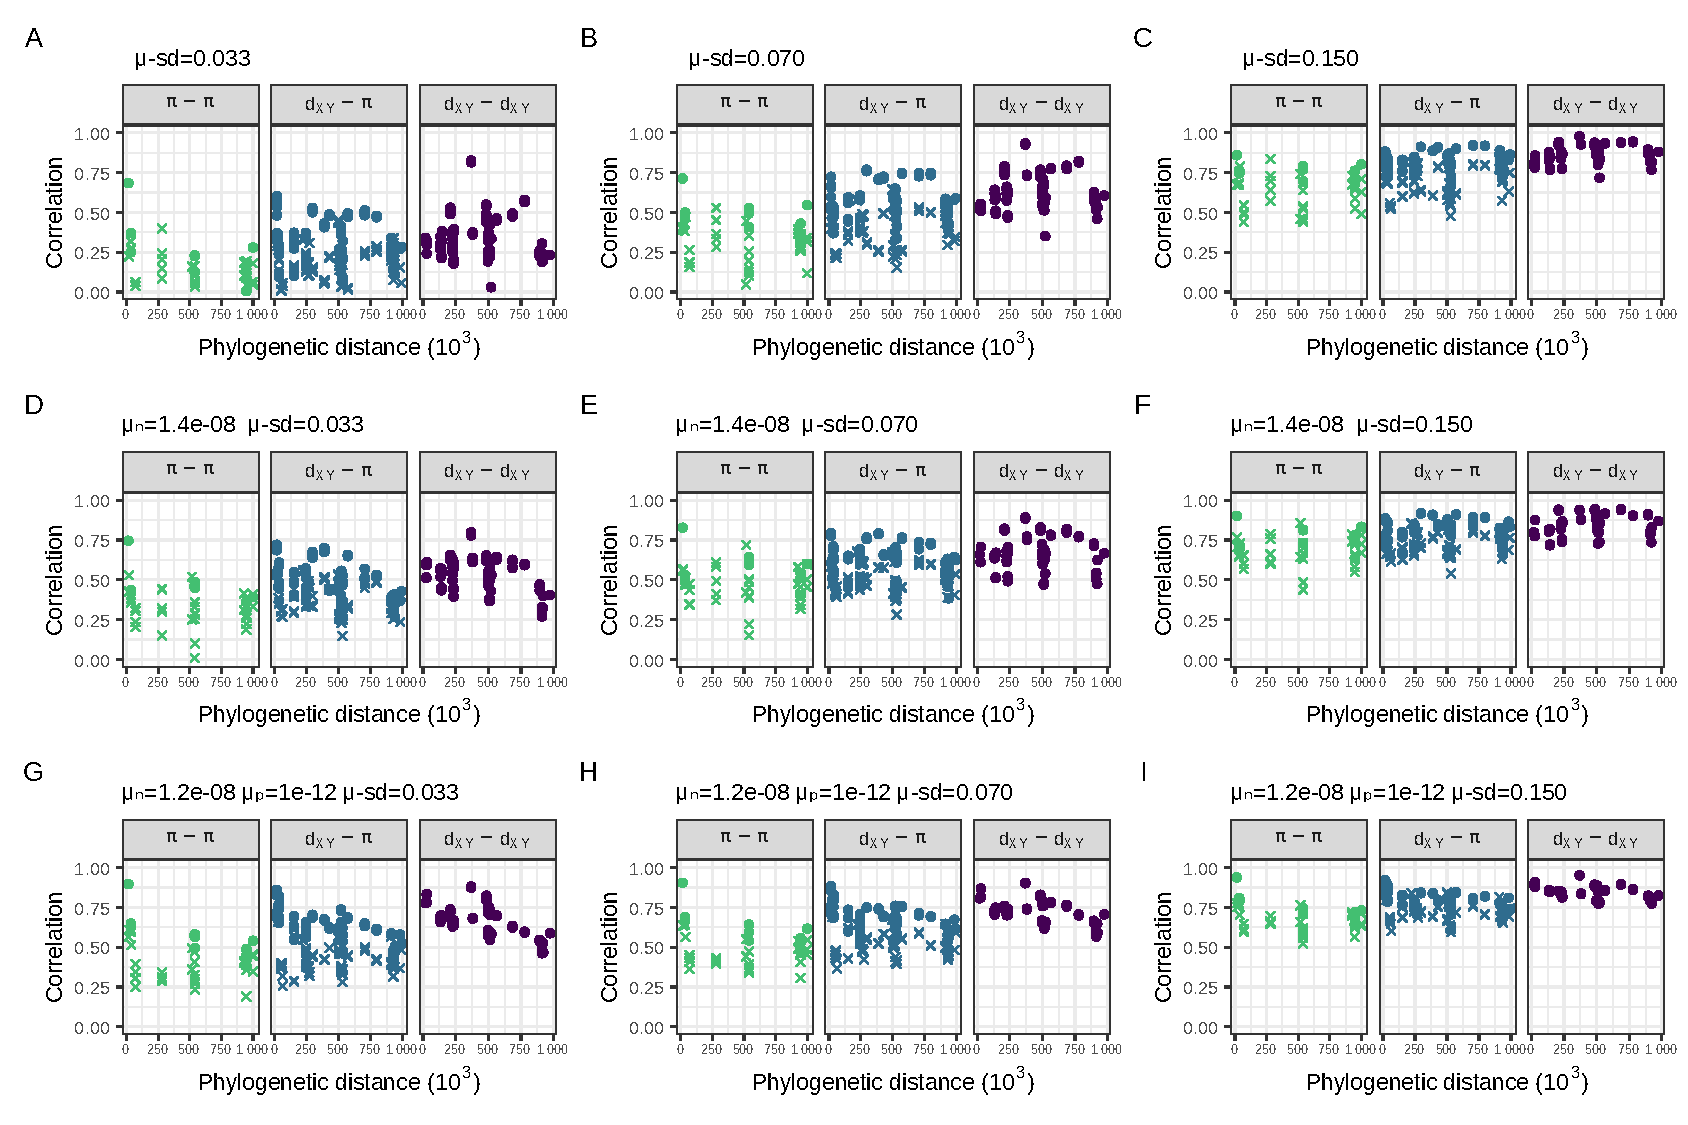
\includegraphics[width=\linewidth]{{figures/cor-pidxy-dT_selected-mutvar-sims.pdf}}
\centering
\caption[Correlations between landscapes of diversity and divergence across the great apes for simulations with variation in mutation rate along the chromosome]{
Correlations between landscapes of diversity and divergence across the great apes for simulations with variation in mutation rate along the chromosome.
Panels A, B, C, and D show different simulations in which we varied the standard deviation in mutation rate between 1Mb windows,
in each setting the standard deviation to the mean mutation rate ($\expnumber{2}{-8}$) multiplied by $\mu_{\SD}$.
Other details are as in \lcref{fig:land_cors}.
}
\label{fig:mutvar_land_cors}
\end{figure}

\subsection{GC-biased gene conversion}

A prominent feature of the landscapes of divergence in the great apes 
is the faster accumulation of divergence in the ends of the chromosomes \plcref{fig:chr12_landscapes}.
This feature was not present in any of our simulations, so we sought to understand its possible causes.
Double strand breaks are more common at the ends of chromosomes, and
these can be repaired either by crossover or gene conversion events.
GC-biased gene conversion (gBGC), the process whereby weak alleles (A and T) are replaced by strong alleles (G and C) in the repair of double-stranded breaks in heterozygotes,
mimics positive selection -- in that it increases the probability of fixation of G and C alleles \citep[e.g.,][]{galtier_gc-biased_2009}.
We suspected gBGC could have caused the increased rate of accumulation divergence in the ends of chromosomes,
as has been observed previously \citep{katzman_gc-biased_2010}, and
contributes to the maintenance of correlations between landscapes over long time scales.

To tease apart the effects of gBGC on correlated landscapes,
we partitioned divergence by mutation type (weak to weak, strong to strong and weak to strong).
If correlations are being driven by gBGC,
then we would expect the correlation between landscapes of divergence to be stronger for weak to strong mutations.
We found that the overall correlations are very similar across mutation types,
suggesting gBGC does not play a strong role in structuring the correlations between landscapes \plcref{fig:partitioned_dxy}.


\begin{figure}[htp]
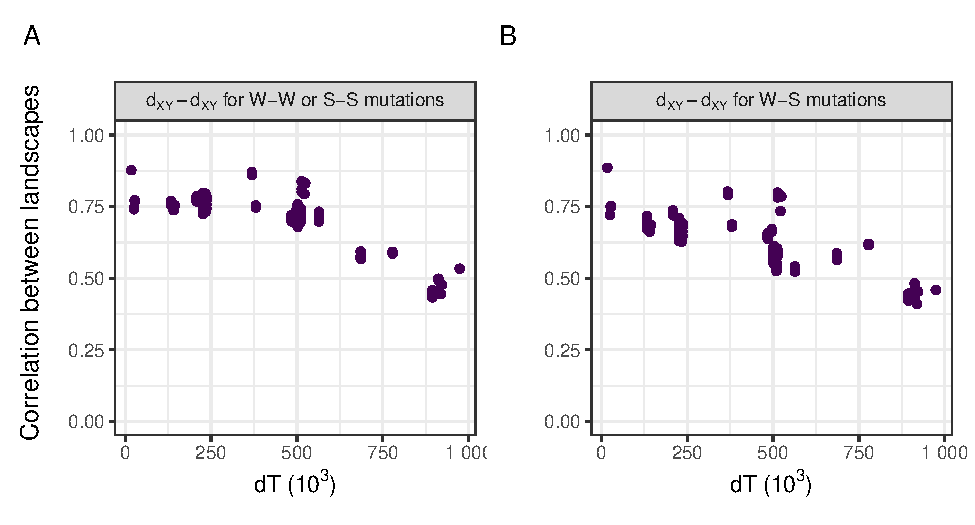
\includegraphics[]{{figures/curr-partitioned-dxydxy-corr_data.pdf}}
\centering
\caption[Correlations between landscapes of divergence partitioned by site type (W-W/S-S and W-S)]{
Correlations between landscapes of divergence partitioned by site type (W-W/S-S and W-S).
W-W sites are sites in which the state did not change between-species (and remained weak which corresponds to A or T).
Similar logic applies to S-S sites (S or strong states are G or C).
W-S sites are sites in which a new mutation appeared either going from weak to strong or from strong to weak.
Note these definitions do not rely on identifying the exact ancestral state, we simply compare the current states in the four species involved (two species per $d_{XY}$ landscape).
For example, if by looking at the four species we see the following states A,T,A,T the site would be classified as W-W.
If we saw G,A,A,A the site would be classified as W-S.
Other details are the same as in the rightmost panel in \lcref{fig:land_cors}.
}
\label{fig:partitioned_dxy}
\end{figure}

\subsection{Positive and negative natural selection}

Another process whose intensity is likely correlated across all branches in the great apes tree is natural selection.
If targets of selection and recombination maps are shared across species, then we would expect both the direct and indirect effects of selection to be shared across branches.
It can be difficult to model natural selection in a realistic manner because we do not know precisely which locations of the genome are subject to stronger selection. 
Nevertheless, exons are expected to have higher density of functional mutations than other places in the genome.
Thus, we ran simulations in which beneficial and deleterious mutations can happen only within exons.
Using human annotations, we simulated the great apes' history assuming a common recombination map and exon locations.
See the landscapes from the simulations in \lcref{fig:sims_land_cors}.

We found that negative selection can slightly increase correlations between landscapes \plcref{fig:sims_land_cors}[A-C].
If $30\%$ of all mutations within exons were strongly deleterious (mean selection coefficient $\bar{s} = -0.03$),
landscapes would be weakly correlated \plcref{fig:sims_land_cors}[B].
The correlations between landscapes rarely surpass $0.5$, even with $70\%$ of all mutations within exons being strongly deleterious \plcref{fig:sims_land_cors}[C].

Positive selection, on the other hand, can quickly increase correlations between landscapes.
A beneficial mutation rate within exons of $\bar{\mu_p}=\expnumber{1}{-12}$
produced moderate correlations between landscapes \plcref{fig:sims_land_cors}[D].
With too much positive selection, 
correlations can break down because of the contrasting effects of positive selection on diversity and divergence.
That is, while positive selection increases fixation rates and hence divergence between-species, its linked effects decrease diversity within the species.
This can create negative correlations between landscapes, as can be seen in \lcref{fig:sims_land_cors}[F].
Note that some correlations between landscapes of diversity and divergence remain high 
when the divergence is computed between closely related species (\eg central and eastern chimps).
Divergence is $d_{XY} = \pianc + 2rT$, 
where $\pi_{\mathrm{anc}}$ is diversity in the ancestor, $r$ is the substitution rate and $T$ is the time since species split.
Thus, for the divergences in which the two species split recently are dominated by genetic diversity in the ancestor, correlations between $\pi-d_{XY}$ remain high because $d_{XY} \simeq \pianc$.

Positive and negative selection can work synergistically to produce correlated landscapes that look like the real data.
For example, comparing figures \lcref{fig:sims_land_cors}[D,G,H] which differ in rate of negatively selected mutations $\mu_n$,
it is possible to see that the correlations between landscapes start to resemble the real data with more deleterious mutations.
\lcref{fig:sims_land_cors}[H] seems to resemble the data fairly well, with $\pi-d_{XY}$ and $d_{XY}-d_{XY}$ correlations plateauing around $0.5$.
The $\pi-\pi$ correlations are a bit lower than the real data, however. 
Recent demographic events can affect genetic diversity and although our simulations are heavily parameterized with respect to the effects of selection,
we are not capturing all the variation caused by more realistic demographic models.
\lcref{fig:sims_land_cors}[D and H] look very similar to each other.
These have the same amount of positive selection, but the first did not have any negative selection.
The major difference between them is that with negative selection there is a more clear separation between the correlations involving low $N_e$ species,
similar to what is seen in the data.

\begin{figure}[htp]
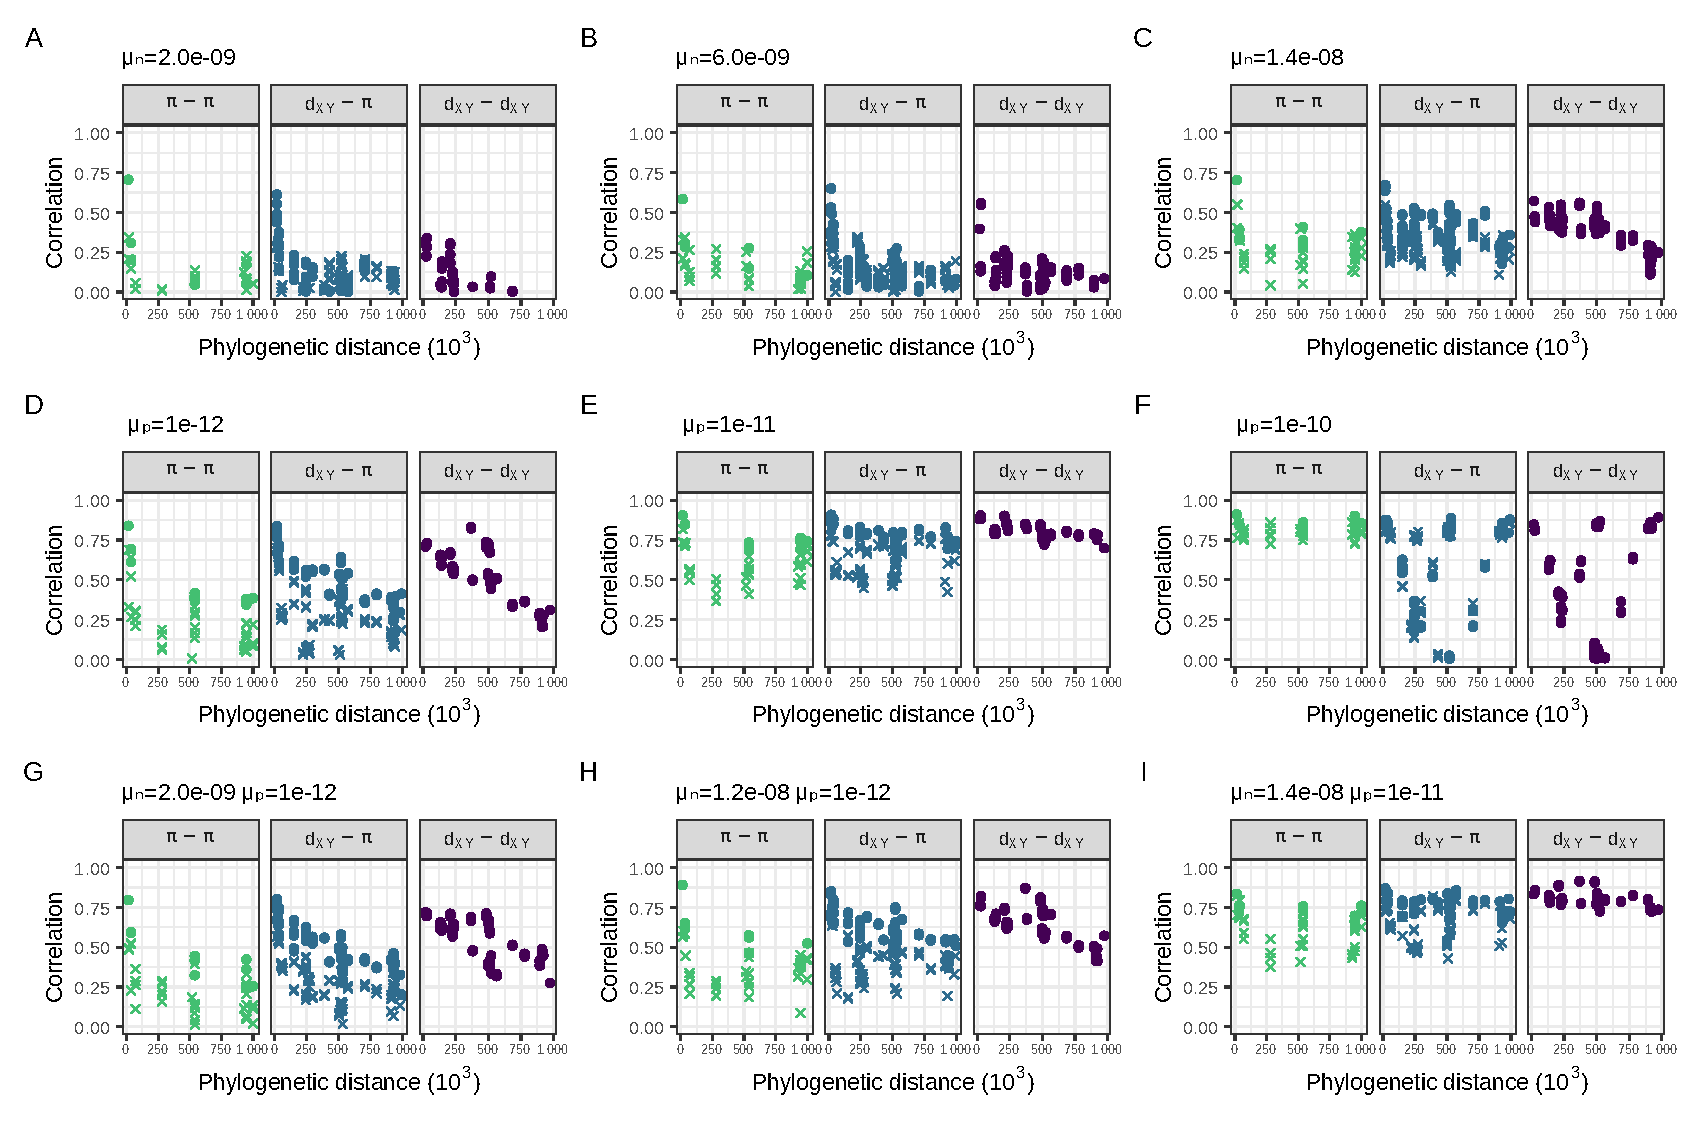
\includegraphics[width=\linewidth]{{figures/cor-pidxy-dT_selected-sel-sims.pdf}}
\centering
\caption[Correlations between landscapes of diversity and divergence in simulations with natural selection]{
Correlations between landscapes of diversity and divergence in simulations with natural selection.
(A-C) Simulations with negative selection.
(D-F) Simulations with positive selection.
(G-I) Simulations with both negative and positive selection. 
The selection parameters $\mu_n$ and $\mu_p$ are the rate of mutations in exons with negative and positive fitness effects, respectively.
The mean fitness effect was $\bar{s}=-0.03$ for deleterious mutations and $\bar{s}=0.01$ for beneficial mutations (see \autoref{sec:methods:simu} for more details).
Compare to \lcref{fig:land_cors}.
}
\label{fig:sims_land_cors}
\end{figure}

\subsection{Visualizing similarity between simulations and data}

To see how a particular simulation resembles the real data, we can use figures \lcref{fig:land_cors} and \lcref{fig:sims_land_cors}
to compare how the patterns of all 1260 pairwise correlations between landscapes match the real data.
However, it is difficult to assess the fit of the simulated scenarios to real data from such a comparison.
Instead, we use principal component analysis (PCA) and create a low dimensional visualization,
shown in \lcref{fig:pca}, in which each point is a simulation or the real data (shown in yellow).
We created this PCA from the matrix $37\times1260$ in which rows are the simulations and the data, and columns are the pairwise Spearman correlations between landscapes.
Unlike in the plots above, here we include the correlations between overlapping landscapes (as detailed in \autoref{sec:methods:visualizing}) \plcref{fig:pca}.
In PC space,
the data most closely resembles a subset of our simulations with both positive and negative selection ($\bar{\mu_p}=\expnumber{1}{-12}$ and $\bar{\mu_n}=\expnumber{1.2}{-8}$) 



\begin{figure}[htp]
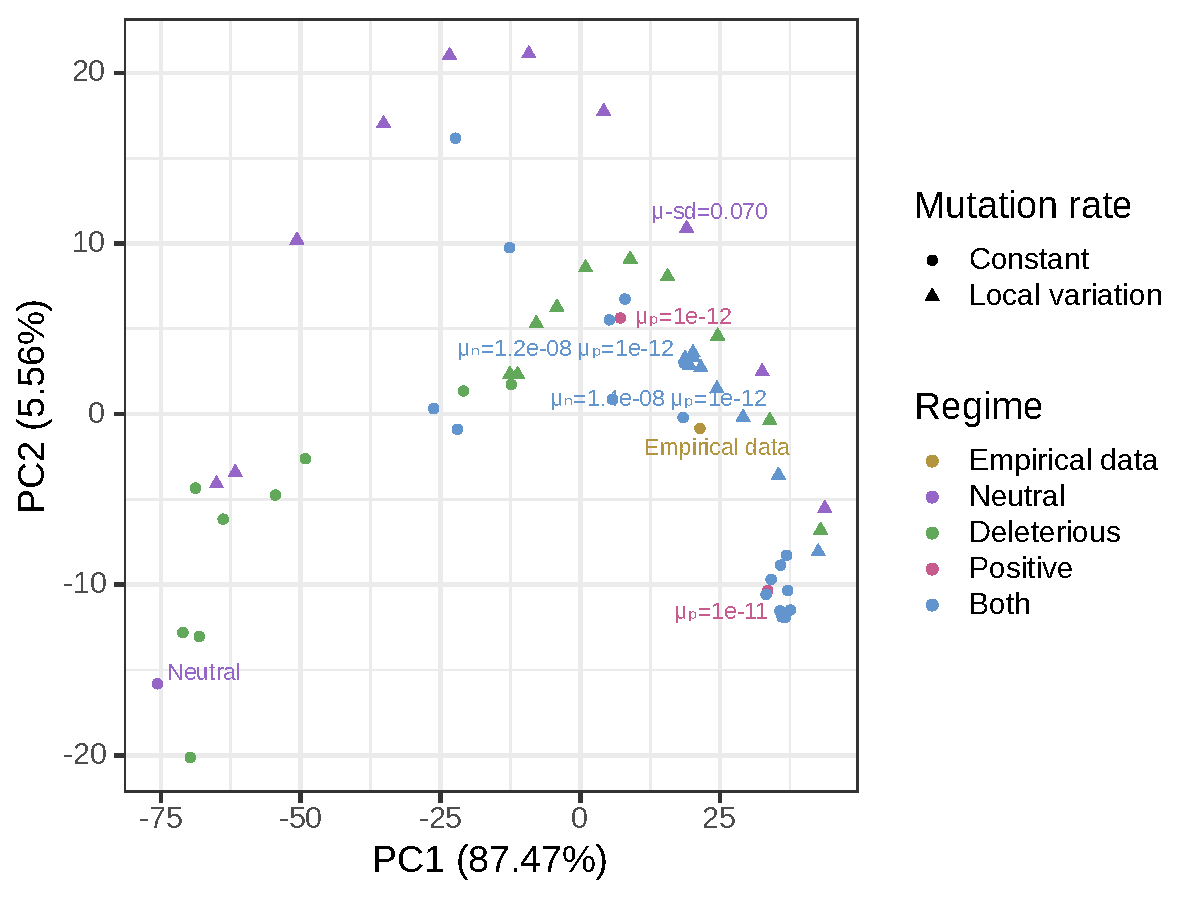
\includegraphics[width=0.7\linewidth]{{figures/data-and-sims_pca.pdf}}
\centering
\caption[PCA visualization of data and simulations]{
PCA visualization of data and simulations.
The colors differentiate the empirical data from simulations with different parameters: Neutral refers to the simulation without any selection, BGS refers to simulations with deleterious mutations, Sweeps refers to simulations with beneficial mutations, Both refers to simulations with both beneficial and deleterious, and MRV refers to neutral simulations with variable mutation rates along the chromosome.
Principal component analysis (PCA) applied to a matrix with all pairwise correlations between landscapes across the great apes 
(including $\pi-\pi$, $\pi-d_{XY}$ and $d_{XY}-d_{XY}$ comparisons) for the great apes dataset and simulations (with selection and with mutation rate variation).
We excluded simulations with $\mu_p \geq \expnumber{1}{-10}$ from the PCA analysis because PC2 was capturing negative correlations caused by strong positive selection --- as seen in \lcref{fig:sims_land_cors}[F].
}
\label{fig:pca}
\end{figure}

\subsection{Correlations between genomic features and diversity and divergence}

Next, we describe how two important genomic features (\ie exon density and recombination rate)
are related to diversity and divergence in the real great apes data set.
The correlations between recombination rate and genetic diversity are positive in all great apes \plcref{fig:annot_cors}[A].
The strongest correlation between genetic diversity and recombination rate is seen in humans, 
which is unsurprising given our recombination map was estimated for humans.
Recent demographic events also seem to impact the strength of the correlation;
for example, the correlation between recombination rate and diversity is higher in Nigerian chimps than in western chimps,
which have a much lower recent effective population size.
We found that diversity is negatively correlated with exon density across all species \plcref{fig:annot_cors}[D].
Contrary to what we observed with recombination rate, 
the correlation between exon density and diversity was even stronger in most other apes than in humans.
Species with smaller $N_e$ tend to show weaker correlation between diversity and exon density (see \citet{nam_evidence_2017} for related findings).
A striking feature of the correlations of between-species divergence and genomic features, shown in \plcref{fig:annot_cors},
is that the correlations get stronger with the amount of phylogenetic time that goes into the comparison (\ie the $T_{MRCA}$),
in a way that is roughly linear with time. 

To describe why this increase in correlation with time might occur, we turn to an analytic approach.
Genetic divergence ($D$) in the $i^\text{th}$ window between two species that split $t$ generations ago can be decomposed as:
$$D_i(t) = \pi_i(t) + R_i t + \varepsilon_i,$$
where $\pi_i(t)$ is the genetic diversity in the ancestor at time $t$, 
$R_i$ is the substitution rate in the window and $\varepsilon_i$ is a contribution from genealogical and mutational noise (which has mean zero). 
This decomposition follows from the definition of genetic divergence as the number of mutations since the common ancestor,
as depicted in \lcref{fig:conceptual_tree} (see how $D_{VX} = \pianc + 2RT_{VWXY}$).
% The genetic diversity in the ancestor in the $i^\text{th}$ window might roughly be modeled as proportional to the effective population size of the ancestor:
% $$\pi_i(t) = N_e(t) \nu_i,$$
% where $N_e(t)$ is the effective population size of the ancestor and $\nu_i$ is the relative diversity of that window in the ancestor.

The covariance between $D(t)$, the vector of divergences along windows, and a genomic feature $X$
is, using bilinearity of covariance,
\begin{align}
    \Cov(D(t),X) &= \Cov(\pi(t), X) + t\Cov(R,X) + \Cov(\varepsilon, X) \label{eqcov} . % \\
                % &= N_e(t) \Cov(\nu, X) + t\Cov(R,X) + \Cov(\varepsilon, X). 
\end{align}
Happily, this equation predicts the linear change of the covariance with time that is seen in \lcref{fig:annot_cors}[C] and perhaps \lcref{fig:annot_cors}[D].
However, caution is needed because the correlation between diversity and the genomic feature ($\Cov(\pi(t), X)$)
may be different in different ancestors,
and indeed the inferred effective population size is greater in older ancestors in the great apes \plcref{fig:sim_demog}.

Next consider covariances of diversity with recombination rate, \lcref{fig:annot_cors}[C].
Consulting the equation above,
the fact that the covariance between divergence and recombination rate increases with time
can be caused by two factors (taking $X$ to be the vector of mean recombination rates along the genome):
(i) a positive covariance between substitution rates and recombination rates ($\Cov(R,X)>0$), and/or
(ii) greater genetic diversity in longer ago ancestors ($N_e(t)$ larger for larger $t$).
It is unlikely that the increase in $N_e$ in more ancient ancestors
was sufficient to produce the dramatic increase in covariance seen in \lcref{fig:annot_cors}[C],
since it would require $\Cov(\pi(t), X)$ to be far larger in the ancestral species
than is seen in any modern species.
On the other hand, there are various plausible mechanisms that would affect $\Cov(R, X)$.
One factor that certainly contributes is the ``smile'':
we found that divergence increases faster near the ends of the chromosomes
where recombination rate is greater,
probably in part because of GC-biased gene conversion.
Interestingly, positive and negative selection are predicted to have opposite effects here:
greater recombination rate increases the efficacy of both through reduced interference among selected alleles,
so positive selection would increase substitution rate and hence increase $\Cov(R, X)$,
while negative selection would decrease $\Cov(R, X)$.
When considering only the middle half of the chromosome (\ie excluding the effect of gBGC) \plcref{fig:annot_cors_center},
the covariances between divergence and recombination rate flip to negative, and they continue to decrease over time.
Thus, it seems that negative selection is the most important driver of divergence in the middle, whereas
gBGC strongly affects the tails of the chromosome.

The covariance of diversity and exon density has a less clear pattern (\lcref{fig:annot_cors}[C]),
although it generally gets more strongly negative with time.
This decrease could be a result of
a negative covariance between substitution rates and exon density
and/or an increase in the population sizes of the ancestors
(if $\Cov(\nu, X) < 0$, as expected since $\nu$ is relative diversity and $X$ is now exon density).
As before, positive selection in exons would be expected to produce a positive covariance
between exon density and substitution rate,
while negative selection would produce a negative covariance.
It is hard to determine \emph{a priori} which is likely to be stronger,
because although negative selection is thought to be much more ubiquitous,
a small amount of positive selection can have a strong effect on substitution rates.
The fact that covariance generally goes down with time
suggests that negative selection (i.e., constraint)
is more strongly affecting substitution rates.

It is at first surprising that the correlations between exon density and divergence go up with time,
but the covariances go down with time \plcref{fig:annot_cors}[E,F].
However, correlation is defined as $\Cor(D_t,X) = \Cov(D_t,X) / \SD(D_t)\SD(X)$.
Thus, if the variance in divergences increases over time
the correlations will decrease over time.
Indeed, we see this happening as gBGC increases divergences on the ends of the chromosome
faster than in the middle, leading to an increase in variance of divergence along the genome.
This also explains why correlations of landscapes of very recent times are very noisy,
but covariances are not.
Indeed, the patterns are clearer when we exclude the tails of the chromosome \plcref{fig:annot_cors_center}:
there is only a modest increase in the correlation between exon density and divergence over time and the covariances go down with time more linearly.



\begin{figure}[htp]
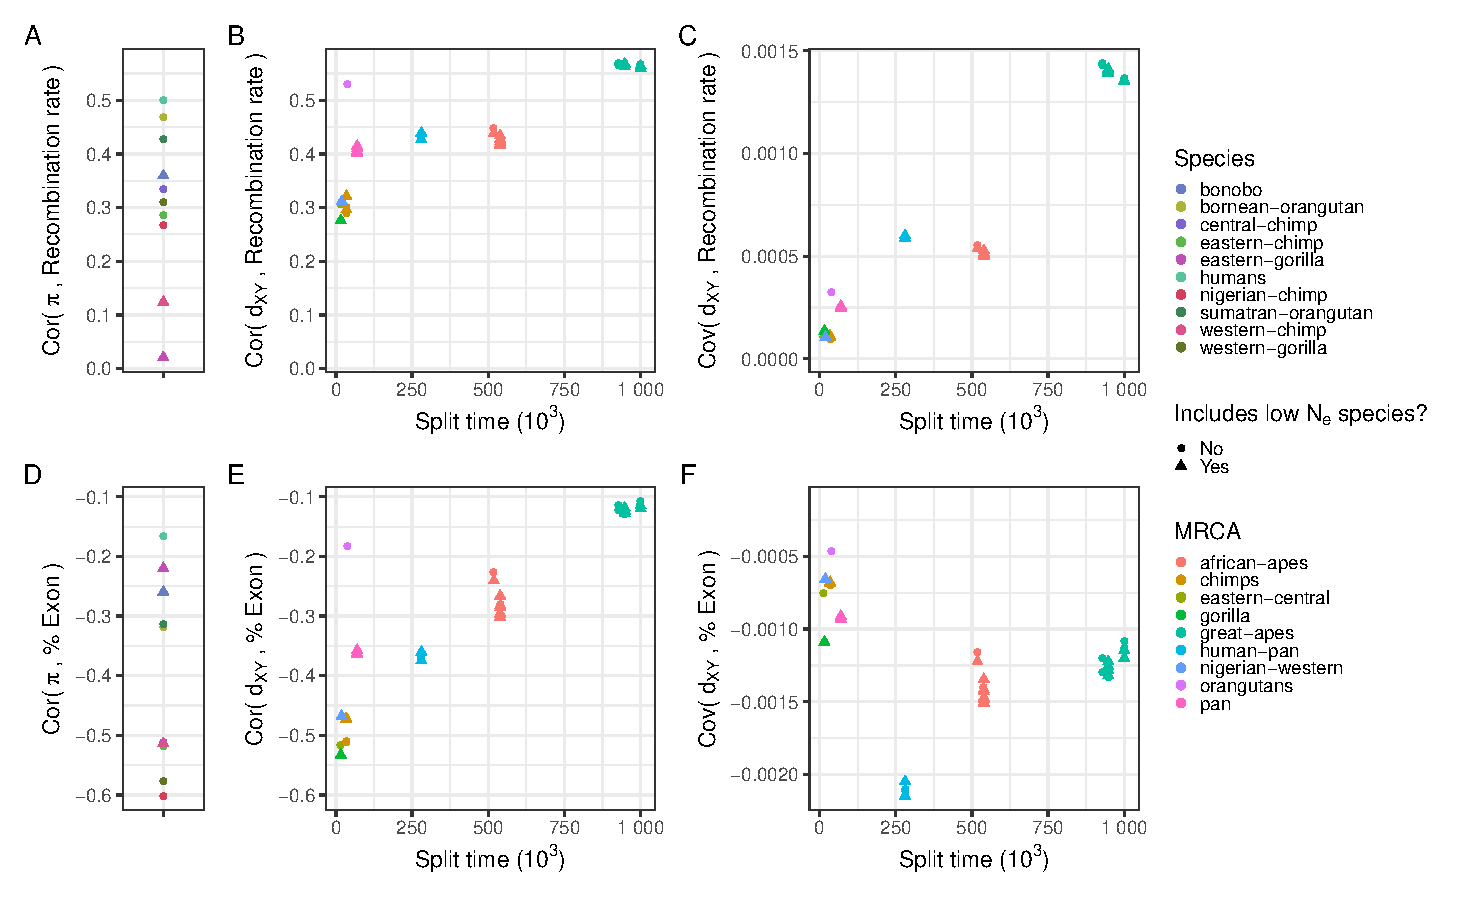
\includegraphics[width=\linewidth]{{figures/cor-pidxy-annot_data.pdf}}
\centering
\caption[Correlations and covariances between landscapes of diversity and divergence and annotation features in the real great apes data]{
Correlations and covariances between landscapes of diversity and divergence and annotation features in the real great apes data.
Exon density and recombination rates were obtained as detailed in \lcref{fig:chr12_landscapes}.
Split time is the time distance between the two species involved in the divergence.
Points are colored by the species of within-species diversity ($\pi$) in plots A and D.
In plots B,C,E,F, the points are colored by the most common recent ancestor of the species for which between-species divergence was computed.
Species with low $N_e$ --- for which the estimated species $N_e$ was less than $\expnumber{8}{3}$: bonobos, eastern gorillas and western chimps --- have a different point shape. 
}
\label{fig:annot_cors}
\end{figure}


\section{Discussion}

A central goal of population genetics is to understand the balance of 
evolutionary forces at work in shaping the origin and maintenance of variation 
within and between-species \citep{lewontin_genetic_1974}.
While the field has been historically data-limited, with the current flood of
genome sequencing data, we are poised to make progress on such old questions.
Over the past decades, an important lever in understanding the relative impact
of genetic drift versus selection in shaping genomic patterns of variation has
been to examine the relationship between \textit{levels} of diversity and 
genomic features, such as recombination rate and exon density.
The overarching observation has been that regions of reduced crossing over
generally harbor less variation than regions of increased crossing over in
many but not all species \parencite[\eg][]{begun_levels_1992, corbett-detig_natural_2015}.
This observation is consistent with a role for linked selection
shaping patterns of variation in recombining genomes,
but  the relative contributions of deleterious and
beneficial mutations is still largely unknown.
Indeed, it seems likely that some complex mixture of both processes shapes variation
in natural populations \parencite{kern_neutral_2018}.

In this paper,
we moved beyond genetic diversity within a single species to look at how divergence between closely related species changes with time
and how this correlates with genomic features.
Previous studies \citep[\eg][]{stankowski_widespread_2019} looked at similar patterns (in monkeyflowers)
and found strong correlations
between landscapes of diversity and divergence between related species, despite deep split 
times.
Landscapes of closely related species can remain correlated for two main reasons (i) shared ancestral variation 
or (ii) shared heterogeneous process.
If two species recently split, their landscapes of diversity are 
expected to be correlated due to shared ancestral variation.
If the process that structures genetic diversity along chromosomes is 
heterogeneous and somewhat shared between-species, then their landscapes are
expected to remain correlated over longer periods of time.
For example, if the effects of selection are concentrated in the same genomic 
regions in two species, then their landscapes of diversity will be correlated.
By incorporating information from multiple species at once,
we are able to pool information across species and thus increase our power to disentangle the role of different evolutionary forces.
Patterns across multiple species are more likely to be robust to the idiosyncrasies of any one species,
such as demographic history.
For instance within-species metrics can be confounded by demography:
demographic events can create spurious troughs of diversity \citep{simonsen_properties_1995} or exacerbate the effects of background selection on diversity \citep{torres_human_2018}.
However, correlations between landscapes can only be produced by shared ancestral variation or shared heterogeneous process.


In the great apes, we found that landscapes of within-species diversity and between-species divergence are 
highly correlated across the phylogeny.
Those correlations are often stronger than those that have been historically used as evidence for the effects of selection on genetic variation.
For example, the correlation between genetic diversity in humans and exon density is $-0.2$, 
yet the correlation between diversity in humans and diversity in western gorillas is $0.48$.
This stronger correlation may not be entirely due to shared landscape of selection --- it may also be a result of shared ancestral variation (\ie incomplete lineage sorting), mutation rate variation,
and/or GC-biased gene conversion.
To understand how much of the correlation between landscapes can be attributed to ancestral variation,
we performed extensive simulations of the great apes' evolutionary history,
and found that ancestral variation explains very little of the correlations we observed.
Thus, a shared heterogeneous process seems to be needed to explain the data.

Two neutral processes can be heterogeneous along the genome and shared across species:
GC-biased gene conversion and mutation.
GC-biased gene conversion (gBGC) is thought to be an important factor in shaping levels of variation in humans \citep{chen_gene_2007, pouyet_background_2018, glemin_quantification_2015},
and it has similar effects to those of natural selection.
However, if gBGC were a major driver of correlations we would expect to see a difference in overall levels
of correlation between different classes of substitution, and we do not \plcref{fig:partitioned_dxy,fig:anc-partitioned_dxy}.
As such gBGC seems to be a minor contributor to the correlations we observe,
although it does seem to be leading to increased substitution rates
near the telomeres
(where divergences are increasing roughly $5\%$ faster; see \lcref{fig:chr12_landscapes} and \lcref{fig:pidxy-change}).
In birds,  an excess of divergence near telomeres has been attributed to meiotic drives \citep{ellegren_genomic_2012}.

When the history of the great apes is simulated with a shared heterogeneous mutation map,
correlations between landscapes do emerge.
These were as strong as seen in the data when the rates were drawn from a normal distribution
with a standard deviation of the mutation rate of at least a 7.7\% of the mean mutation rate.
However, our mutation map was perfectly shared among was species in our simulations,
so it is possible that a mutation map which changes over time might move closely to match the data.
Mutation rate varies along the human genome 
and \citet{smith_large_2018} estimated the standard deviation of de novo mutation rate in humans at the 1Mb scale to be above 25\% (with respect to the mean).
However, this prior estimates of variation in de novo mutation rate did not take into account differences in callability along genomes
-- due to the fact that genomic regions vary in how well they can be genotyped with short-read data --
which can bias inference.
Our simulations showed a facet of shared mutational heterogeneity along the genome
that we do not observe in real data: with variable mutation rate correlations increase over time,
whereas in the real data they decrease.
It is unknown how conserved mutation rate heterogeneity is across the great apes,
so it remains to be seen how an evolving heterogeneous mutation rate map affects landscapes of diversity and divergence.
A major driver of mutation rate variation stems from CpG dinucleotides,
which have much higher mutation rates than other sites \citep{agarwal_mutation_2021, nachman_estimate_2000, hodgkinson_variation_2011}.
Nevertheless, when we partitioned the landscapes of divergence by mutation types,
we did not see an excess of correlation between landscapes with mutations
that can be affected by CpG-induced mutation rate variation \plcref{fig:partitioned_dxy,fig:anc-partitioned_dxy}.

Natural selection can also structure genetic variation heterogeneously along the genome.
In simulations,
both positive and negative selection are needed for the correlations between landscapes to resemble the data.
We chose exons to be the targets of selection in our simulations.
Exons cover about $1\%$ of the human genome, 
but in reality selection is known to affect non-coding regions as well.
For example, highly conserved noncoding sequences have long been identified
and characterized as functional \citep{bejerano_ultraconserved_2004, siepel_evolutionarily_2005, katzman_human_2007}.
Therefore, we might expect a more realistic model to have the same amount of selection (in terms of total influx of selected mutations),
but spread out over a somewhat wider region of the genome since we have omitted such sites.
While that is so, conserved noncoding sequences generally occur close to coding regions
of the genome.
By examining the correlations between landscapes (summarized in \lcref{fig:pca}),
we found that the best fitting simulation is the one with a beneficial mutation rate within exons of $\expnumber{1}{-12}$ and deleterious rate within exons of $\expnumber{1.4}{-8}$.
Our results largely agree with previous studies which found that positive selection is necessary to explain reduction in genetic diversity surrounding genes in the great apes \citep{nam_extreme_2015, nam_evidence_2017}.

Another way we might characterize our simulations is 
through examination of substitution processes.
In our best fitting simulation, 
we get a fixation rate of beneficial mutations of around $\expnumber{1}{-9}$ per generation per exon base pair,
what amounts to around $10\%$ of the fixations within exons (along the human lineage) and
about one new fixation of a beneficial mutation every 250 generations.
Total fixation rate is decreased by around $55\%$ relative to the rate in our neutral simulation due to the constant removal of deleterious mutations within exons.
Indeed, previous studies \citep{boyko_assessing_2008} have estimated that around 10\% of amino acid differences between humans and chimpanzees were caused by positive selection,
strikingly similar to our best fitting simulation.
Furthermore, we would expect to see the fixation of around 16 beneficial mutations in the past 4000 generations,
which is close to the number of hard sweeps genome scans for selections have found in humans over this same time period \citep{schrider_soft_2017, schrider_shic_2016}.
Our best fitting simulation with selection assumes that $70\%$ of mutations within exons are deleterious,
similar to estimates from the site frequency spectrum \citep{boyko_assessing_2008,kim_inference_2017, huber_determining_2017}.
Thus while we have not done exhaustive model fitting due to computational constraints, our simulations recapitulate
major patterns of variation observed in the genome.

Heterogeneous processes that correlate with a genomic feature
will create differences in rates of substitution along the genome
that correlate with the genomic feature.
As shown in \Cref{eqcov}, this implies that 
the covariance along the genome between a genomic feature and divergence
is expected to increase with time,
and the rate of increase is
equal to the covariance between that feature and the substitution rate.
(It is important to note that
varying covariances with ancestral diversity can be a confounding factor,
and that the observation applies to covariance, not correlation.)
Indeed,
the covariance between divergence and recombination rate increases roughly linearly with time
(see \lcref{fig:annot_cors}{C}),
as expected because the rate of gBGC-induced fixations are correlated with recombination rate.
Once this effect is removed (see \lcref{fig:annot_cors_center}{F}),
the covariance between exon density and divergence decreases linearly with time,
% implying a negative covariance between exon density and substitution rate,
as we would expect due to the effects of negative selection directly removing deleterious mutations
in or near exons.
The magnitude of this slope might produce a quantitative estimate
of the strength of this effect,
although more work is needed to disentangle confounders.
It is important to contrast this observation,
which applies mostly to the direct effects of selection,
to other observations which also include linked effects
(as discussed in \citet{phung_determining_2016}).


While it has long been recognized that genetic variation among species might be
structured similarly due to shared targets of selection, our results demonstrate
that this signal contains important information about the processes at work that has yet to be utilized fully.
Here we have used large-scale simulations to demonstrate the combination of forces required 
to patterns shared divergence and diversity as we observe it in nature, however
there is clearly a need for future analytical work that might describe expected
correlations across the genome given heterogeneous mutation, recombination,
and selection. Further, statistical model fitting, based on theory or
simulation is clearly desirable, although our experience suggests that the latter
approach would prove computationally expensive. 


\newpage
\section{Bridge}

As presented in Chapter III, simulations can be useful to help us distinguish between evolutionary models.
We showed that although many processes are consistent with great apes population genomic data,
positive selection seems necessary to fully explain the observed data.
Beyond qualitative assessments, in many cases we might want to infer parameters from a model.
The evolutionary simulations of the entire great apes history were too costly to allow for proper parameter estimation.
In Chapter IV, we present a new method for simulation-based parameter estimation using whole-genome genealogies.
This method is expected to resolve a different bottleneck that plagues evolutionary inference: the scaling with number of samples and genome sizes.
Whole-genome genealogies are much more efficient than genotype matrices (matrices with dimensions of number of samples by number of sites).
Moreover, they are expected to organize genetic information in a way that can be more conducive for estimating evolutionary parameters.
Our main contribution, a deep learning architecture that takes whole-genome genealogies as input, seems to perform well over different tasks.
More importantly, it could enable evolutionary inference over biobank scale datasets (that contain millions of samples).

\chapter{A powerful machine learning framework for evolutionary inference using whole-genome genealogies} \label{chapter:tsnn}

\bigskip
Nathaniel S. Pope, Peter L. Ralph and Andrew D. Kern are co-authors on this manuscript.
Co-authors and I conceptualized the study,
Nathaniel S. Pope and I developed the machine learning framework,
I performed analyses with input from my co-authors,
I wrote the manuscript with editorial assistance from my co-authors.\\
\bigskip

\section{Introduction}

% Genetic data carries information about past evolutionary events
% Kinds of things that can be inferred from genetic data
% With the increase in population genomic data, there is demand for powerful computational tools that can use the big data
Processes like mutation, recombination, population size changes and selection leave footprints on genetic variation.
A major goal of population genetics has been to invert this relationship and infer past, unobserved evolutionary events from genetic variation data \citep{schraiber_methods_2015}.
However, with the dramatic increase in our ability to generate whole-genome data,
there is a need for more efficient inference methods that can scale well to over tens of thousands of individuals.

% How has inference been done traditionally?
% Thinking about how processes impact trees, then translating that into summary statistics that can be computed from genetic data.
% These stats do lose some information, however.
Historically, evolutionary inference is done on summary statistics of population genetic data.
However, it is simpler to first think about the effects of evolutionary processes on the underlying genealogies \citep{wakely_coalescent_2016},
that is, the trees that describe the relationships between samples of a population.
For example, recent contractions in population sizes will lead to trees which have shorter branches near the tips (due to an increase in the rate of coalescence caused by the contraction).
Although the trees are unknown, it is possible to describe how changes in the shape of genealogies will affect genetic variation.
The site frequency spectrum,
which describes the distrubution of allele frequencies across sites in the genome,
is a statistic that has been succesfully used to infer demographic histories from natural populations \citep{gutenkunst_inferring_2009, schraiber_methods_2015}.
In the example of a recent population size reduction,
we would expect an excess of derived alleles with intermediate and high frequencies,
because most of the coalescences will have occured in the recent past leading to big internal branches where most of the mutations would fall.


% Inference can be done in by computing likelihoods, but these are tricky, specially for some summary stats.
% One can do inference on multiple stats at once using simulation-based inference.
An issue with using summary statistics is that these cannot capture all aspects of variation in genetic data that are informative of the underlying processes.
Some studies have circumvented this by using multiple summary statistics either in a composite likelihood framework or with likelihood-free methods \citep{nielsen_genomic_2005, degiorgio_sweepfinder2_2016, sheehan_deep_2016, caldas_inference_2022, pavlidis_sweed_2013}.
Writing and computing likelihoods in complex evolutionary scenarios can be challenging.
Likelihood-free methods (\eg ABC or machine learning) have gained some popularity in population genetics,
followed by advances in evolutionary genetics simulation software that can be used to generate labeled training data \citep{haller_tree-sequence_2019, kelleher_efficient_2016, ralph_efficiently_2020}.
%Some examples of applications: Sheehan PLoS CompBio, SHIC, Pavlidis, Michael DiGiorgio, etc. 

% Traditional likelihood-free methods have been using genotype matrices or summary stats matrices for inference.
% CNNs on these matrices do well, but there is a problem with scaling (wrt to sampling and genome size).
Many of the likelihood-free methods model how evolutionary processes impact summary statistics along chromosomes (or windows) or raw genotype matrices \citep{schrider_shic_2016, flagel_unreasonable_2019, sheehan_deep_2016}.
When dealing with large chromosomes, these have to be split into chunks for computational tractability;
that is, when the number of loci grows it becomes computationally infeasible to apply these methods over large matrices.
In the case of summary statistics, it is possible to compute them over larger windows to capture variation along full chromosomes,
but this comes at the cost of losing granularity and some evolutionary signals can be quite localized \citep{caldas_inference_2022}.

% An alternative data structure, the whole genome genealogies, can be leveraged for evol inference.
% This structure is way more compact and the data is restructured in such a way that can facilitate learning.
An alternative data structure, whole-genome genealogies, can be leveraged for evolutionary inference.
Genotype matrices are redundant due to shared ancestry, that is related samples will share the same alleles at many of the variant sites.
Trees, which describe the relationships between samples from a population, provide a more efficient way of encoding genetic data.
In recombining genomes, there is not a single tree, but rather a collection of trees (which are autocorrelated) along chromosomes.
Recent work has made it possible to infer whole-genome genealogies for thousands of individuals \citep{speidel_inferring_2021, kelleher_inferring_2019, zhang_biobank-scale_2023}.

Benefits of these tree sequences go beyond computational efficiency and scallability, however.
Trees can perfectly encode evolutionary processes and event and can bring us closer to the processes that we are interested in inferring \citep{rasmussen_genome-wide_2014}.
Indeed, much of population genetics inference starts from understanding how a particular process impacts the underlying genealogies.
More than that, trees bring a time dimension which can be helpful in inferring events localized in time (\eg migration pulses, past selective sweeps, etc.) \citep{speidel_inferring_2021}.

Here, we present a new method that leverages these whole-genome genealogies for evolutionary inference.
Our main goal is to develop an architecture that can efficiently use genealogies for inference,
which can be done at different scales.

% Here, we aim to develop an architecture that uses these whole genome genealogies for inference.

\section{Methods} \label{sec:methods}

\subsection{Simulations}

\subsection{Model}

\subsection{Tasks}

\section{Results and discussion}

\subsection{Inferring mutation times}

\subsection{Inferring demographic model parameters}

\section{Conclusion}


\chapter{Conclusion}

Understanding the balance of evolutionary forces shaping the origin and maintenance of genetic variation has been the core driver of population genetics \citep{lewontin_genetic_1974}.
Our ability to collect data has exponentially increased over the last few decades, moving from allozyme gels of a few samples to whole-genome data of thousands of individuals.
With this flood of data, we are poised to make huge progress on long standing evolutionary questions.
However, the traditional framework for evolutionary inference has somewhat stalled new discoveries.

Many of the issues we are facing can be mitigated with evolutionary simulations.
A great deal of progress has been made on evolutionary simulation tools \citep{haller_slim_2019,kelleher_efficient_2016, haller_tree-sequence_2019,adrion_community-maintained_2020}.
These advancements, coupled with huge increases in computational power, now allow us to use simulations to effectively infer previously intractable likelihoods,
and to explore features of the data that are not easy to model mathematically.
Indeed, over the past decade simulation-based inference has gained immense popularity \citep{schrider_shic_2016,torres_human_2018,caldas_inference_2022,chan_likelihood-free_2018,korfmann_simultaneous_2023}.

% importance of standards and reproducibility
As the questions and models increase in complexity, 
there is a growing need for standards in simulation models and for increase reproducibility.
\stdpopsim is a community-maintained library for previously published simulation models, 
which includes species-specific population genetic parameters (\eg mutation rates, recombination maps) as well as demographic and selection models.
Much more is needed still in two fronts:
(i) benchmarking our current tools under a common variety of evolutionary scenarios, and
(ii) verifying for consistency of published models, for example by ensuring that the models can yield simulated data that actually resembles the real data.

% arg and inference
The move from 
The adoption of a common data structure across evolutionary simulation tools, the tree sequence, 

% some remaining issues

% outlook 


%------------------------------------------------------------------------------%
% APPENDICES
%------------------------------------------------------------------------------%
\appendix
% Changes the table and figure counting to A.1 style
\renewcommand\thefigure{\thechapter.\arabic{figure}}
\renewcommand\thetable{\thechapter.\arabic{table}}

%--- Appendix A ---------------------------------------------------------------%
\chapter{The First Appendix}
\section{Appendix One Section One}
\subsection{Chapter four section one sub-section one}

%--- Appendix B ---------------------------------------------------------------%
% Restart counting to B.1, B.2...
\setcounter{figure}{0}
\setcounter{table}{0}
\chapter{The Second Appendix}
\section{Appendix Two Section One}
\subsection{Chapter two section one sub-section one}



\printbibliography{}


\end{document}
%==============================================================================%
% END DOCUMENT
%==============================================================================%
